% ============================================================
%  Forces and Motion — Lesson Booklet (one section per lesson: A Reading · B Theory · C Practice · D Above level)
%  Years 7–8  |  Victorian Curriculum F–10 Version 2.0
%  Compile with: xelatex, three times (see CLAUDE.md) --- fill.py does this and sizes the answer boxes
%
%  TWO BUILDS FROM THIS ONE SOURCE (the Ch3G-L / Trebuchet pattern)
%    Forces_Motion_Lesson_Booklet_Yr7_8.tex          student copy --- no answers
%    Forces_Motion_Lesson_Booklet_Yr7_8_Teacher.tex  teacher copy --- defines
%        \teacheranswers (every \defans, read from teacher-answers/L01.tex ...
%        L14.tex, plus \teacherappendix) and then \input's this file, so every
%        box, cell, drawing space and graph prints its model answer in red.
%  The teacher wrapper, teacher-answers/ and the teacher PDF are gitignored:
%  answer keys never ship as a plain file (ROADMAP.md, "Staff material").
%  Keep this file free of answers. A key missing from the wrapper prints
%  ??key?? in the teacher copy, so grep the teacher PDF for "??" after a build.
%
%  Every answer-bearing piece of furniture carries a key: \abox{key}{h} (ruled
%  writing box), \wbox{key}{h} (plain box for calculations), \rcqk{key}{q}{h}
%  (comprehension Cn), \cell{key} (write-in table cell), \drawk{key}{h}{caption}
%  and \graphgrid{key}{h}. Keys were set from the printed numbering on
%  30 Oct 2026 (6.t3b = Task 6.3(b), 6.x9 = Extension 6.9, 6.c2 = C2,
%  6.wd1a = We do 6.1(a), 6.pred = prediction, 6.v3 = vocab row 3,
%  6.res-r2c3 = results table row 2 column 3) and are literal from then on:
%  renumbering the booklet never moves an answer. New furniture needs a new key.
%
%  Both copies paginate identically: answers sit inside fixed-height boxes and
%  cells. The teacher build reads the STUDENT page-fill file (.abx) and never
%  writes one, so build the student copy (and run fill.py) first. Both builds
%  log every key with its page and printed label to <jobname>.akp; the two
%  files must agree page for page (tools/forces_solutions.py checks this).
% ============================================================
\documentclass[11pt,a5paper,twoside]{article}
\newcommand{\unitname}{Advanced Forces}\newcommand{\unitcaps}{ADVANCED FORCES}

% ── Student / teacher switch ─────────────────────────────────────────────────
% The teacher wrapper defines \teacheranswers (every \defans) before \input-ing
% this file. Without it this is the student copy and every answer is blank.
\newif\ifteacher
\makeatletter
\newcommand{\defans}[2]{\@namedef{kans@#1}{#2}}
\newcommand{\getans}[1]{\@ifundefined{kans@#1}{\textbf{??#1??}}{\@nameuse{kans@#1}}}
\newcommand{\hasans}[1]{\@ifundefined{kans@#1}{\@secondoftwo}{\@firstoftwo}}
\makeatother
\ifdefined\teacheranswers \teachertrue \teacheranswers \fi
% Page-fill files always use the student copy's name, so the teacher build
% reads the student layout and never writes its own.
\providecommand\abbase{\jobname}

% ── Fonts (compile with XeLaTeX) ────────────────────────────────────────────
\usepackage{fontspec}
% Bundled fonts (in ./fonts/) so the document compiles anywhere with XeLaTeX/LuaLaTeX
\setmainfont{Lato}[                   % body — humanist sans (stands in for deck's Inter)
  Path=../fonts/, Extension=.ttf, Ligatures=TeX,
  UprightFont=Lato-Regular, ItalicFont=Lato-Italic,
  BoldFont=Lato-Bold, BoldItalicFont=Lato-BoldItalic ]
\newfontfamily\headingfont{Poppins}[  % display/headings — matches the slide decks
  Path=../fonts/, Extension=.ttf, Ligatures=TeX,
  UprightFont=Poppins-Regular, ItalicFont=Poppins-Italic,
  BoldFont=Poppins-Bold, BoldItalicFont=Poppins-BoldItalic ]
\setlength{\headheight}{22pt}

\usepackage[protrusion=true,expansion=false]{microtype}
\usepackage[a5paper, inner=17mm, outer=13mm, top=19mm, bottom=17mm, headheight=14pt, headsep=4mm, footskip=8mm]{geometry}
\usepackage{xcolor}
\usepackage{tikz}
\usetikzlibrary{arrows.meta, shapes.geometric, calc, positioning, decorations.pathreplacing}
\usepackage{tcolorbox}
\tcbuselibrary{skins, breakable, raster}
\usepackage{fancyhdr}
\usepackage{titlesec}
\usepackage{enumitem}
\usepackage{booktabs}
\usepackage{tabularx}
\usepackage{array}
\usepackage{colortbl}
\usepackage{multicol}
\usepackage{amsmath}
\usepackage{needspace}
% TikZ diagram macros are embedded below (just before \begin{document}) for easy editing.
\usepackage{longtable}
\usepackage{graphicx}
\usepackage{lastpage}
\usepackage{calc}
\usepackage{mdframed}
\usepackage{setspace}
\usepackage{ragged2e}
% PDF bookmarks: one per lesson (made in \sectiondiv) plus the cover and
% contents, and links from the contents table to each lesson.
% implicit=false: hyperref adds no anchors of its own (an anchor on each
% list item nudged lists down 1.5 mm, which would undo the page fill).
% hidelinks keeps the links invisible, so the printed pages are unchanged.
\usepackage[implicit=false, hidelinks,
  pdftitle={Forces and Motion — Lesson Booklet},
  pdfsubject={Years 7–8 Science, Victorian Curriculum F–10 v2.0}]{hyperref}
\usepackage{bookmark}
\makeatletter\providecommand\Hy@PageAnchorSlide{}\makeatother % writes the outline itself, which implicit=false switches off in hyperref

% ── Colour Palette ───────────────────────────────────────────────────────────
% Remapped to the slide-deck palette (names kept so body + diagrams cascade)
\definecolor{NavyBlue}   {HTML}{16305C}
\definecolor{MidBlue}    {HTML}{2E6FE0}
\definecolor{LightBlue}  {HTML}{E8F1FF}
\definecolor{TealGreen}  {HTML}{0F6E63}
\definecolor{LightGreen} {HTML}{E0F7F3}
\definecolor{GoldDark}   {HTML}{C77F12}
\definecolor{GoldLight}  {HTML}{FFF3DC}
\definecolor{PurpleDark} {HTML}{5B3FC0}
\definecolor{PurpleLight}{HTML}{EFE9FF}
\definecolor{OrangeDark} {HTML}{C9483D}
\definecolor{OrangeLight}{HTML}{FFE9E6}
\definecolor{MidGrey}    {HTML}{AEBED4}
\definecolor{LightGrey}  {HTML}{F2F5FA}
\definecolor{DarkGrey}   {HTML}{3A4759}
\definecolor{TableHead}  {HTML}{16305C}
\definecolor{RowAlt}     {HTML}{EEF4FF}
% Bright accent tints (deck) for bars, rules and chips
\definecolor{Blue}   {HTML}{2E6FE0}
\definecolor{Teal}   {HTML}{18A999}
\definecolor{Amber}  {HTML}{F5A623}
\definecolor{Coral}  {HTML}{FF6B5E}
\definecolor{Violet} {HTML}{7C5CE0}
\definecolor{Sky}    {HTML}{4DA3FF}
\definecolor{Ink}    {HTML}{16223A}
\definecolor{Line}   {HTML}{DDE5F0}
\definecolor{Paper}  {HTML}{FBFCFE}

% ── Page Style ───────────────────────────────────────────────────────────────
\pagestyle{fancy}
\fancyhf{}
\renewcommand{\headrulewidth}{0.4pt}
\renewcommand{\headrule}{\hbox to\headwidth{\color{NavyBlue}\leaders\hrule height \headrulewidth\hfill}}
\fancyhead[L]{\headingfont\small\color{NavyBlue}Forces and Motion}
\fancyhead[R]{\headingfont\small\ifteacher\textcolor{ScaffoldRed}{\bfseries Teacher copy}\ \textbar{}\ \fi\color{DarkGrey}Years 7--8 \textbar{} Victorian Curriculum F--10 v2.0}
\fancyfoot[C]{\headingfont\small\color{DarkGrey}\thepage\ \textbar{} \pageref{LastStudentPage}}
\fancypagestyle{plain}{%
  \fancyhf{}
  \fancyfoot[C]{\headingfont\small\color{DarkGrey}\thepage\ \textbar{} \pageref{LastStudentPage}}
  \renewcommand{\headrulewidth}{0pt}
}

% ── Section Formatting ───────────────────────────────────────────────────────
\titleformat{\section}
  {\headingfont\color{NavyBlue}\Large\bfseries}
  {}{0em}{}
  [{\color{Teal}\rule[0.6ex]{2.2em}{3pt}}{\color{Line}\rule[0.6ex]{\dimexpr\linewidth-2.2em\relax}{1pt}}]
\titlespacing{\section}{0pt}{18pt}{8pt}

\titleformat{\subsection}
  {\headingfont\color{MidBlue}\large\bfseries}
  {\thesubsection}{0.6em}{}
\titlespacing{\subsection}{0pt}{12pt}{4pt}

\titleformat{\subsubsection}
  {\headingfont\color{NavyBlue}\normalsize\bfseries}
  {}{0em}{}
\titlespacing{\subsubsection}{0pt}{8pt}{2pt}

% Deck-style eyebrow / kicker (optional use)
\newcommand{\kicker}[2][Teal]{%
  {\headingfont\bfseries\footnotesize\color{#1}%
   \textcolor{#1}{\rule[0.18ex]{1.6em}{2.2pt}}\hspace{0.5em}\MakeUppercase{#2}\par}%
  \vspace{2pt}}

% ── Custom tcolorbox Environments ────────────────────────────────────────────

% Section divider banner
\newtcolorbox{sectionbanner}[2]{
  enhanced, breakable=false,
  colback=NavyBlue, colframe=NavyBlue,
  fontupper=\color{white}\bfseries\large,
  left=4mm, right=4mm, top=3mm, bottom=3mm,
  title={\color{white}\Huge\bfseries #1},
  attach boxed title to top left={yshift=-2mm, xshift=4mm},
  boxed title style={colback=NavyBlue, colframe=NavyBlue},
  after upper={\par\smallskip\normalfont\normalsize\color{white!80!NavyBlue}\textit{#2}}
}

% Key info box (blue)
\newtcolorbox{infobox}[1]{
  breakable, arc=2.5mm, boxrule=0.5pt,
  colback=LightBlue, colframe=Blue!40,
  fonttitle=\headingfont\bfseries, coltitle=MidBlue,
  title={#1},
  left=4mm, right=3.5mm, top=2.5mm, bottom=2.5mm
}

% Scaffold box (yellow)
\newtcolorbox{scaffold}[1]{
  before upper={\anslabelset{Prediction}},
  breakable, arc=2.5mm, boxrule=0.5pt,
  colback=GoldLight, colframe=Amber!40,
  fonttitle=\headingfont\bfseries, coltitle=GoldDark,
  title={#1},
  left=4mm, right=3.5mm, top=2.5mm, bottom=2.5mm
}

% Worked example box
\newtcolorbox{workedexbox}[1]{
  breakable, arc=2.5mm, boxrule=0.5pt,
  colback=white, colframe=Amber!50,
  fonttitle=\headingfont\bfseries, coltitle=GoldDark,
  title={#1},
  left=4mm, right=3.5mm, top=2.5mm, bottom=2.5mm
}
% Worked examples: \begin{workedex}{title} -> "Worked Example N.M --- title",
% auto-numbered per section and labelled we:N.M. Never type the number.
\newcounter{wenum}[section]
\renewcommand{\thewenum}{\thesection.\arabic{wenum}}
\newenvironment{workedex}[1]
  {\refstepcounter{wenum}\label{we:\thewenum}\begin{workedexbox}{Worked Example \thewenum\ --- #1}}
  {\end{workedexbox}}

% We do: straight after each worked example, a near-identical question the
% class works through together, with its own writing space. Numbered to
% match the worked example above it and labelled wd:N.M.
%   \begin{wedo}{title} question ... \answerbox{h} \end{wedo}
\newtcolorbox{wedobox}[1]{
  enhanced, breakable=false, arc=2.5mm, boxrule=0.5pt,
  colback=white, colframe=TealGreen!55,
  fonttitle=\headingfont\bfseries, coltitle=TealGreen!75!black,
  title={#1},
  left=4mm, right=3.5mm, top=2.5mm, bottom=2.5mm
}
\newenvironment{wedo}[1]
  {\par\needspace{9\baselineskip}\anslabelset{We do \thewenum}\begin{wedobox}{We do \thewenum\ --- #1}\label{wd:\thewenum}\ignorespaces}
  {\end{wedobox}}

% Year 7 box (blue)
\newtcolorbox{yr7box}{
  breakable, arc=2.5mm, boxrule=0.5pt,
  colback=LightBlue, colframe=Blue!40,
  left=4mm, right=3.5mm, top=2.5mm, bottom=2.5mm
}

% Year 8 extension box (violet)
\newtcolorbox{yr8box}{
  breakable, arc=2.5mm, boxrule=0.5pt,
  colback=PurpleLight, colframe=Violet!40,
  left=4mm, right=3.5mm, top=2.5mm, bottom=2.5mm
}

% Answer lines box
\newcommand{\answerbox}[1]{%
  \begin{tcolorbox}[
    enhanced, breakable, arc=2mm,
    colback=Paper, colframe=Line,
    left=2mm, right=2mm, top=1mm, bottom=1mm,
    boxrule=1pt,
    height=#1
  ]
  \end{tcolorbox}%
}

% Experiment header
\newtcolorbox{expheader}[3]{
  breakable=false, arc=2.5mm,
  colback=RowAlt, colframe=Amber!50, boxrule=0.5pt,
  fonttitle=\headingfont\bfseries\large, coltitle=NavyBlue,
  title={Experiment #1: #2},
  left=4mm, right=3.5mm, top=2.5mm, bottom=2.5mm,
  after upper={\par\smallskip
    {\headingfont\bfseries\color{GoldDark}Aim:}\ \textit{#3}},
}

% Reading comprehension passage box (green)
\newtcolorbox{readingbox}[1]{
  breakable, arc=2.5mm, boxrule=0.5pt,
  colback=white, colframe=Teal!50,
  fonttitle=\headingfont\bfseries, coltitle=TealGreen,
  title={#1},
  left=4mm, right=3.5mm, top=2.5mm, bottom=2.5mm,
  fontupper=\normalsize
}

% Skill-builder box (for beginner scaffolding)
\newtcolorbox{skillbox}[1]{
  breakable, arc=2.5mm, boxrule=0.5pt,
  colback=RowAlt, colframe=Blue!40,
  fonttitle=\headingfont\bfseries, coltitle=MidBlue,
  title={#1},
  left=4mm, right=3.5mm, top=2.5mm, bottom=2.5mm
}

% ── Custom Commands ───────────────────────────────────────────────────────────

% Question: \question{marks}{text}  (marks can be empty)
% Numbered automatically as Q<section>.<n>, reset every section.
% Do NOT write numbers by hand.
\newcounter{qnum}[section]
\renewcommand{\theqnum}{\thesection.\arabic{qnum}}
\newcommand{\question}[2]{%
  \refstepcounter{qnum}%
  \needspace{3\baselineskip}%
  \medskip
  \noindent\label{q:\theqnum}\textbf{Q\theqnum}\ifx&#1&\else\ \textcolor{DarkGrey}{(#1 mark\ifnum#1=1\else s\fi)}\fi\quad #2%
  \medskip
}

% Inline marks note
\newcommand{\markscount}[1]{\hfill\textcolor{DarkGrey}{\textit{(#1 mark\ifnum#1=1\else s\fi)}}}

% ── Practice set counter and question macros ─────────────────────────────────
\newcounter{pqnum}
\newcommand{\practiceset}[1]{%
  \needspace{6\baselineskip}
  \setcounter{pqnum}{0}%
  \vspace{6pt}
  {\headingfont\bfseries\large\color{GoldDark} Practice Set --- #1}\\[-2pt]
  {\color{Amber}\rule{\linewidth}{1pt}}\\[2pt]
}
% \pq{question text}{working box height}
\newcommand{\pq}[2]{%
  \stepcounter{pqnum}%
  \needspace{4\baselineskip}
  \vspace{5pt}
  \noindent\textbf{\thepqnum.}\quad #1\par
  \vspace{2pt}
  \answerbox{#2}
}
% Two short questions side by side, each with its own box
\newcommand{\pqpair}[4]{%
  \needspace{4\baselineskip}
  \vspace{5pt}
  \noindent
  \begin{minipage}[t]{0.48\linewidth}
    \stepcounter{pqnum}\textbf{\thepqnum.}\quad #1\par\vspace{2pt}
    \begin{tcolorbox}[enhanced,arc=2mm,colback=Paper,colframe=Line,left=2mm,right=2mm,
      top=1mm,bottom=1mm,boxrule=1pt,height=#2]\end{tcolorbox}
  \end{minipage}\hfill
  \begin{minipage}[t]{0.48\linewidth}
    \stepcounter{pqnum}\textbf{\thepqnum.}\quad #3\par\vspace{2pt}
    \begin{tcolorbox}[enhanced,arc=2mm,colback=Paper,colframe=Line,left=2mm,right=2mm,
      top=1mm,bottom=1mm,boxrule=1pt,height=#4]\end{tcolorbox}
  \end{minipage}
}

% ── Comprehension question macro (compact, lined) ────────────────────────────
\newcounter{rcnum}
\newcommand{\rcreset}{\setcounter{rcnum}{0}}
\newcommand{\rcq}[2]{%
  \stepcounter{rcnum}%
  \needspace{3\baselineskip}
  \vspace{4pt}
  \noindent\textbf{C\thercnum.}\quad #1\par
  \vspace{2pt}
  \answerbox{#2}
}

% Section divider (big numbered banner): \sectiondiv{title}{summary}
%
% This IS the section: it steps the real section counter, so subsections,
% tasks, questions and figures inside it are numbered N.M automatically.
% Put \label{sec:N} straight after it. Never hand-type a section number.
\newcommand{\sectiondiv}[2]{%
  \needspace{5\baselineskip}%
  \refstepcounter{section}%
  % PDF bookmark for the lesson; its anchor, lesson.N.1, is what the contents table links to
  \pdfbookmark[1]{Lesson \thesection{} — #1}{lesson.\thesection}%
  \begin{tcolorbox}[
    enhanced, breakable=false, arc=3.5mm,
    colback=NavyBlue, colframe=NavyBlue, boxrule=0pt,
    sidebyside, sidebyside align=center,
    lefthand width=2.0cm,
    left=2mm, right=4mm, top=4mm, bottom=4mm
  ]
    \begin{center}
      {\headingfont\bfseries\color{white!35!NavyBlue}\fontsize{50}{50}\selectfont \thesection}
    \end{center}
    \tcblower
    {\headingfont\bfseries\color{white}\LARGE #1}\\[3pt]
    {\itshape\color{white!75!NavyBlue}\small #2}
  \end{tcolorbox}%
}

% Tasks: \task, \task[a] (part a of a NEW task), \taskpart{b} (next part
% of the same task), \exttask (Year 8 "Extension" — same counter).
% Numbered Task <section>.<n>, reset every section. Do NOT type numbers.
% Every task, question and figure also gets an automatic label
% (task:1.7b, q:2.4, fig:1.2, fig:E2.1) so page refs come from the .aux.
\newcounter{tasknum}[section]
\renewcommand{\thetasknum}{\thesection.\arabic{tasknum}}
\NewDocumentCommand{\task}{o}{\refstepcounter{tasknum}\label{task:\thetasknum\IfValueT{#1}{#1}}\textbf{Task \thetasknum\IfValueT{#1}{#1}}}
\newcommand{\taskpart}[1]{\label{task:\thetasknum#1}\textbf{Task \thetasknum#1}}
\newcommand{\exttask}{\refstepcounter{tasknum}\label{task:\thetasknum}\textbf{Extension \thetasknum}}

% Figure captions: \figcap[fig:label]{caption} -> "Figure N.M --- caption"
% \expfigcap{caption} -> "Figure EN.M" (experiment pages). Both auto-numbered.
\newcounter{fignum}[section]
\renewcommand{\thefignum}{\thesection.\arabic{fignum}}
\newcounter{expfignum}[section]
\renewcommand{\theexpfignum}{E\thesection.\arabic{expfignum}}
\newcommand{\figcap}[2][]{%
  \begin{center}
    \refstepcounter{fignum}\label{fig:\thefignum}\if\relax\detokenize{#1}\relax\else\label{#1}\fi
    \small\itshape\color{DarkGrey} Figure \thefignum\ --- #2
  \end{center}%
}
\newcommand{\expfigcap}[1]{%
  \begin{center}
    \refstepcounter{expfignum}\label{fig:\theexpfignum}%
    \small\itshape\color{DarkGrey} Figure \theexpfignum\ --- #1
  \end{center}%
}

% Diagram include
\newcommand{\diagramfig}[3]{%  {filename}{width fraction}{caption}
  \begin{center}
    \includegraphics[width=#2\linewidth]{#1}\\[4pt]
    \small\itshape\color{DarkGrey} #3
  \end{center}%
}

% Table column types
\newcolumntype{L}[1]{>{\RaggedRight\arraybackslash}p{#1}}
\newcolumntype{C}[1]{>{\Centering\arraybackslash}p{#1}}

% Table header colour
\newcommand{\thead}[1]{\cellcolor{TableHead}\color{white}\bfseries #1}
\newcommand{\talt}{\rowcolor{RowAlt}}
\newcommand{\tmid}{\rowcolor{MidGrey}}

% Inline year tags
\newcommand{\tagyr}[1]{%
  \tikz[baseline=-0.5ex]\node[
    rounded corners=2pt,
    fill=#1!20, draw=#1, text=#1,
    inner xsep=4pt, inner ysep=1pt,
    font=\scriptsize\bfseries
  ]{Yr #1 only};}

% Draw answer lines
\newcommand{\anslines}[1]{%
  \vspace{2pt}%
  \foreach \n in {1,...,#1}{%
    \par\noindent\rule{\linewidth}{0.3pt}\vspace{3pt}%
  }%
}

% ── Document ─────────────────────────────────────────────────────────────────
% ══════════════════════════════════════════════════════════════════════════════
%  EMBEDDED DIAGRAM DEFINITIONS  (formerly tikz_diagrams.tex)
%  Edit any figure here; each \diag... macro is called from the body by name.
% ══════════════════════════════════════════════════════════════════════════════
% ============================================================
%  TikZ Diagram Definitions — Forces and Motion Unit Booklet
%  Self-contained macros, no external image files.
%  Requires: tikz with arrows.meta, calc, positioning, patterns
% ============================================================

\usetikzlibrary{arrows.meta,calc,positioning,patterns,backgrounds}

\tikzset{
  force arrow/.style={-{Stealth[length=7pt,width=5pt]}, line width=2pt},
  dim arrow/.style={<->, >=Stealth, thin, color=DarkGrey},
  thin arrow/.style={-{Stealth[length=6pt,width=4pt]}, line width=1.4pt},
  ground hatch/.style={pattern=north east lines, pattern color=DarkGrey!50},
}

% ── D1: Contact vs Non-contact Forces ─────────────────────────────────────────
\newcommand{\diagForceTypes}{%
\begin{center}
\begin{fitbox}\begin{tikzpicture}[font=\small]
  % Contact forces box
  \node[draw=MidBlue, fill=LightBlue, rounded corners=5pt,
        minimum width=5.6cm, minimum height=3.8cm] (cbox) at (0,0) {};
  \node[font=\small\bfseries, text=NavyBlue] at (0, 1.65) {Contact Forces};
  \node[anchor=west, text=NavyBlue, font=\small] at (-2.5, 1.1)  {\textbullet\ Friction};
  \node[anchor=west, text=NavyBlue, font=\small] at (-2.5, 0.65) {\textbullet\ Normal force};
  \node[anchor=west, text=NavyBlue, font=\small] at (-2.5, 0.20) {\textbullet\ Tension};
  \node[anchor=west, text=NavyBlue, font=\small] at (-2.5,-0.25) {\textbullet\ Applied force};
  \node[anchor=west, text=NavyBlue, font=\small] at (-2.5,-0.70) {\textbullet\ Air resistance};
  \node[anchor=west, text=NavyBlue, font=\small] at (-2.5,-1.15) {\textbullet\ Spring force};
  % Non-contact forces box
  \node[draw=black!55!black, fill=black!8, rounded corners=5pt,
        minimum width=5.6cm, minimum height=3.8cm] (ncbox) at (6.4,0) {};
  \node[font=\small\bfseries, text=black!55!black] at (6.4, 1.65) {Non-contact Forces};
  \node[anchor=west, text=black!55!black, font=\small] at (3.9, 1.1)  {\textbullet\ Gravity};
  \node[anchor=west, text=black!55!black, font=\small] at (3.9, 0.65) {\textbullet\ Magnetic force};
  \node[anchor=west, text=black!55!black, font=\small] at (3.9, 0.20) {\textbullet\ Electrostatic force};
  \node[anchor=west, text=black!55!black, font=\small] at (3.9,-0.25) {\textbullet\ Nuclear force};
\end{tikzpicture}\end{fitbox}
\end{center}}

% ── D2: Free Body Diagrams ────────────────────────────────────────────────────
\newcommand{\diagFBD}{%
\begin{center}
\begin{fitbox}\begin{tikzpicture}[font=\small]
  % ── LEFT: Balanced ──
  \node[font=\small\bfseries, text=NavyBlue] at (0,3.6) {Balanced Forces};
  \fill[ground hatch] (-1.5,-1.0) rectangle (1.5,-0.7);
  \draw[thick, DarkGrey] (-1.5,-0.7) -- (1.5,-0.7);
  \node[draw=MidBlue, fill=LightBlue, rounded corners=3pt,
        minimum width=1.8cm, minimum height=1.0cm,
        font=\small\bfseries, text=NavyBlue] (book) at (0,0) {Book};
  % Normal up
  \draw[force arrow, TealGreen] (book.north) -- ++(0,1.8)
        node[right, font=\small\bfseries, text=TealGreen] {$N=10$\,N};
  % Weight down
  \draw[force arrow, black!65!black] (book.south) -- ++(0,-1.8)
        node[right, font=\small\bfseries, text=black!65!black] {$W=10$\,N};
  \node[font=\footnotesize\itshape, text=DarkGrey] at (0,-3.2) {Net force $= 0$\,N};
  \node[font=\footnotesize\itshape, text=DarkGrey] at (0,-3.65) {No acceleration};

  % ── RIGHT: Unbalanced ──
  \node[font=\small\bfseries, text=NavyBlue] at (7.5,3.6) {Unbalanced Forces};
  \fill[ground hatch] (6.0,-1.0) rectangle (9.0,-0.7);
  \draw[thick, DarkGrey] (6.0,-0.7) -- (9.0,-0.7);
  \node[draw=MidBlue, fill=LightBlue, rounded corners=3pt,
        minimum width=1.8cm, minimum height=1.0cm,
        font=\small\bfseries, text=NavyBlue] (box) at (7.5,0) {Box};
  % Normal up
  \draw[force arrow, TealGreen] (box.north) -- ++(0,1.8)
        node[right, font=\small\bfseries, text=TealGreen] {$N$};
  % Weight down
  \draw[force arrow, black!65!black] (box.south) -- ++(0,-1.8)
        node[right, font=\small\bfseries, text=black!65!black] {$W$};
  % Push right (20N, longer)
  \draw[force arrow, PurpleDark] (box.east) -- ++(2.6,0)
        node[above, font=\small\bfseries, text=PurpleDark] {Push 20\,N};
  % Friction left (5N, shorter)
  \draw[force arrow, OrangeDark] (box.west) -- ++(-1.6,0)
        node[above, font=\small\bfseries, text=OrangeDark] {Friction 5\,N};
  \node[font=\footnotesize\itshape, text=DarkGrey] at (7.5,-3.2) {Net force $= 15$\,N $\rightarrow$};
  \node[font=\footnotesize\itshape, text=DarkGrey] at (7.5,-3.65) {Accelerates rightward};
\end{tikzpicture}\end{fitbox}
\end{center}}

% ── D3: Newton's First Law ─────────────────────────────────────────────────────
\newcommand{\diagNewtonOne}{%
\begin{center}
\begin{fitbox}\begin{tikzpicture}[font=\small]
  % Law statement
  \node[draw=PurpleDark, fill=PurpleLight!50, rounded corners=5pt,
        minimum width=13cm, minimum height=1.1cm, align=center,
        font=\small\bfseries, text=PurpleDark] at (5.5,2.8)
        {\textit{``An object at rest stays at rest, and an object in motion stays in}\\[-1pt]
         \textit{motion, unless acted on by an unbalanced force.''\ (Law of Inertia)}};

  % Ground lines
  \draw[thick, DarkGrey] (-0.4,0) -- (2.2,0);
  \draw[thick, DarkGrey] (3.6,0) -- (7.0,0);
  \draw[thick, DarkGrey] (8.5,0) -- (11.5,0);

  % Ball 1: at rest
  \shade[ball color=MidBlue!80] (0.9,0.42) circle (0.42);
  \node[font=\footnotesize\bfseries, text=NavyBlue] at (0.9,1.9) {At rest};
  \draw[force arrow, TealGreen]   (0.9,0.84) -- (0.9,1.5);
  \draw[force arrow, black!65!black](0.9,0.0)  -- (0.9,-0.65);
  \node[font=\scriptsize, text=TealGreen, right]    at (0.9,1.2)  {$N$};
  \node[font=\scriptsize, text=black!65!black, right] at (0.9,-0.3) {$W$};
  \node[font=\scriptsize\itshape, text=DarkGrey] at (0.9,-1.1) {stays at rest};

  % Arrow 1→2
  \draw[-{Stealth}, thick, DarkGrey!60] (2.4,-2) -- (3.4,-2)
        node[midway, above, font=\scriptsize\itshape, text=DarkGrey] {no force added};

  % Ball 2: rolling
  \shade[ball color=TealGreen!70] (5.3,0.42) circle (0.42);
  \node[font=\footnotesize\bfseries, text=TealGreen] at (5.3,1.9) {Rolling (no friction)};
  \draw[force arrow, MidBlue] (5.72,0.42) -- (7.0,0.42)
        node[above, font=\scriptsize, text=MidBlue] {$v$};
  \node[font=\scriptsize\itshape, text=DarkGrey] at (5.3,-1.1) {keeps moving};

  % Arrow 2→3
  \draw[-{Stealth}, thick, DarkGrey!60] (7.4,-2) -- (8.3,-2)
        node[midway, above, font=\scriptsize\itshape, text=DarkGrey] {force applied};

  % Ball 3: stopping
  \shade[ball color=MidBlue!80] (9.9,0.42) circle (0.42);
  \node[font=\footnotesize\bfseries, text=black!60!black] at (9.9,1.9) {Unbalanced force};
  \draw[force arrow, black!65!black] (9.48,0.42) -- (8.4,0.42)
        node[above, font=\scriptsize, text=black!65!black] {friction};
  \node[font=\scriptsize\itshape, text=DarkGrey] at (9.9,-1.1) {decelerates / stops};
\end{tikzpicture}\end{fitbox}
\end{center}}

% ── D4: Newton's Second Law — F=ma ────────────────────────────────────────────
\newcommand{\diagFma}{%
\begin{center}
\begin{fitbox}\begin{tikzpicture}[font=\small]
  \node[draw=PurpleDark, fill=PurpleLight!50, rounded corners=5pt,
        minimum width=13cm, minimum height=0.9cm, align=center,
        font=\small\bfseries, text=PurpleDark]
        at (5.5,3.6)
        {Newton's Second Law: \quad $F = m \times a$ \quad $\Rightarrow$ \quad
         $a = F/m$ \quad $\Rightarrow$ \quad $m = F/a$};
  \node[draw=GoldDark, fill=GoldLight, rounded corners=5pt,
        minimum width=3.6cm, minimum height=3.2cm, align=center]
        at (0.8,1.5)
        {\textbf{\color{GoldDark}$F$\ (Force)}\\[4pt]
         \small\color{DarkGrey}Measured in newtons (N)\\
         \small\color{DarkGrey}A push or pull\\[2pt]
         \small\color{GoldDark}$F = m \times a$};
  \node[font=\large\bfseries, text=DarkGrey] at (3.3,1.5) {$=$};
  \node[draw=MidBlue, fill=LightBlue, rounded corners=5pt,
        minimum width=3.6cm, minimum height=3.2cm, align=center]
        at (5.5,1.5)
        {\textbf{\color{MidBlue}$m$\ (Mass)}\\[4pt]
         \small\color{DarkGrey}Measured in kg\\
         \small\color{DarkGrey}More mass\,=\,more\\
         \small\color{DarkGrey}inertia to overcome};
  \node[font=\large\bfseries, text=DarkGrey] at (7.75,1.5) {$\times$};
  \node[draw=TealGreen, fill=LightGreen, rounded corners=5pt,
        minimum width=3.6cm, minimum height=3.2cm, align=center]
        at (10.0,1.5)
        {\textbf{\color{TealGreen}$a$\ (Acceleration)}\\[4pt]
         \small\color{DarkGrey}Measured in m/s$^2$\\
         \small\color{DarkGrey}Bigger $F$ on same\\
         \small\color{DarkGrey}mass\,=\,bigger $a$};
\end{tikzpicture}\end{fitbox}
\end{center}}

% ── D5: Energy Types and Transformation ───────────────────────────────────────
\newcommand{\diagEnergy}{%
\begin{center}
\begin{fitbox}\begin{tikzpicture}[font=\small]
  % Top row: three energy type boxes
  \node[draw=GoldDark, fill=GoldLight, rounded corners=5pt,
        minimum width=4.0cm, minimum height=2.2cm, align=center]
        at (0.0,3.2)
        {\textbf{\color{GoldDark}Kinetic Energy (KE)}\\[3pt]
         \small\color{DarkGrey}Energy of motion\\[2pt]
         \small\color{GoldDark}$KE = \tfrac{1}{2}mv^2$};
  \node[draw=MidBlue, fill=LightBlue, rounded corners=5pt,
        minimum width=4.0cm, minimum height=2.2cm, align=center]
        at (4.8,3.2)
        {\textbf{\color{MidBlue}Gravitational PE}\\[3pt]
         \small\color{DarkGrey}Stored by height\\[2pt]
         \small\color{MidBlue}$GPE = mgh$};
  \node[draw=TealGreen, fill=LightGreen, rounded corners=5pt,
        minimum width=4.0cm, minimum height=2.2cm, align=center]
        at (9.6,3.2)
        {\textbf{\color{TealGreen}Elastic PE}\\[3pt]
         \small\color{DarkGrey}Stored by stretching\\[2pt]
         \small\color{DarkGrey}springs, rubber bands};
  % Divider label
  \node[font=\small\bfseries, text=DarkGrey] at (4.8,1.85)
        {Energy Transformation in a Trebuchet};
  % Chain: GPE box
  \node[draw=OrangeDark, fill=OrangeLight, rounded corners=4pt,
        minimum width=3.0cm, minimum height=1.1cm, align=center,
        font=\small\bfseries, text=OrangeDark] (n1) at (0.8,0.7)
        {Gravitational PE\\[-1pt]{\scriptsize\color{DarkGrey}(counterweight up)}};
  % Chain: KE1 box
  \node[draw=GoldDark, fill=GoldLight, rounded corners=4pt,
        minimum width=3.0cm, minimum height=1.1cm, align=center,
        font=\small\bfseries, text=GoldDark] (n2) at (4.8,0.7)
        {Kinetic Energy\\[-1pt]{\scriptsize\color{DarkGrey}(arm swings)}};
  % Chain: KE2 box
  \node[draw=TealGreen, fill=LightGreen, rounded corners=4pt,
        minimum width=3.0cm, minimum height=1.1cm, align=center,
        font=\small\bfseries, text=TealGreen] (n3) at (8.8,0.7)
        {Kinetic Energy\\[-1pt]{\scriptsize\color{DarkGrey}(ball launches)}};
  % Waste box
  \node[draw=DarkGrey, fill=LightGrey, rounded corners=4pt,
        minimum width=2.8cm, minimum height=0.9cm, align=center,
        font=\small, text=DarkGrey] (nw) at (8.8,-0.75)
        {$+$ Thermal \& Sound\\[-1pt]{\scriptsize(wasted)}};
  % Arrows
  \draw[-{Stealth}, thick, DarkGrey] (n1.east) -- (n2.west);
  \draw[-{Stealth}, thick, DarkGrey] (n2.east) -- (n3.west);
  \draw[-{Stealth}, thick, DarkGrey] (n3.south) -- (nw.north);
\end{tikzpicture}\end{fitbox}
\end{center}}

% ── D6: Three Classes of Lever ────────────────────────────────────────────────
\newcommand{\diagLevers}{%
\begin{center}
\begin{fitbox}\begin{tikzpicture}[font=\small]
  % ── Class 1: Fulcrum between E and L ── (effort and load both push down)
  \node[anchor=west, font=\small\bfseries, text=NavyBlue] at (-0.3,5.9) {Class 1: Fulcrum between E and L};
  \node[anchor=east, font=\small\itshape, text=DarkGrey]  at (12.0,5.9) {e.g.\ seesaw, crowbar};
  \draw[line width=4pt, DarkGrey!60, line cap=round] (1.0,4.2) -- (10.5,4.2);
  \fill[black!65!black] (5.5,4.2) -- ++(-.22,-.52) -- ++(.44,0) -- cycle;
  \node[font=\scriptsize\bfseries, text=black!65!black, right] at (5.75,3.9) {F};
  \draw[force arrow, MidBlue]   (1.5,5.05) -- (1.5,4.28);
  \draw[force arrow, TealGreen] (9.5,5.05) -- (9.5,4.28);
  \node[font=\small\bfseries, text=MidBlue,   above] at (1.5,5.05) {E};
  \node[font=\small\bfseries, text=TealGreen, above] at (9.5,5.05) {L};

  % ── Class 2: Load between F and E ── (effort lifts upwards)
  \node[anchor=west, font=\small\bfseries, text=NavyBlue] at (-0.3,3.25) {Class 2: Load between F and E};
  \node[anchor=east, font=\small\itshape, text=DarkGrey]  at (12.0,3.25) {e.g.\ wheelbarrow, nutcracker};
  \draw[line width=4pt, DarkGrey!60, line cap=round] (1.0,1.9) -- (10.5,1.9);
  \fill[black!65!black] (1.0,1.9) -- ++(-.22,-.52) -- ++(.44,0) -- cycle;
  \node[font=\scriptsize\bfseries, text=black!65!black, right] at (1.25,1.6) {F};
  \draw[force arrow, TealGreen] (5.0,2.75) -- (5.0,1.98);
  \node[font=\small\bfseries, text=TealGreen, above] at (5.0,2.75) {L};
  \draw[force arrow, MidBlue]   (9.5,1.0) -- (9.5,1.82);
  \node[font=\small\bfseries, text=MidBlue,   right] at (9.55,1.25) {E};

  % ── Class 3: Effort between F and L ── (effort lifts upwards)
  \node[anchor=west, font=\small\bfseries, text=NavyBlue] at (-0.3,0.35) {Class 3: Effort between F and L};
  \node[anchor=east, font=\small\itshape, text=DarkGrey]  at (12.0,0.35) {e.g.\ tweezers, your forearm};
  \draw[line width=4pt, DarkGrey!60, line cap=round] (1.0,-0.9) -- (10.5,-0.9);
  \fill[black!65!black] (1.0,-0.9) -- ++(-.22,-.52) -- ++(.44,0) -- cycle;
  \node[font=\scriptsize\bfseries, text=black!65!black, right] at (1.25,-1.2) {F};
  \draw[force arrow, TealGreen] (9.5,-0.05) -- (9.5,-0.82);
  \node[font=\small\bfseries, text=TealGreen, left] at (9.45,-0.3) {L};
  \draw[force arrow, MidBlue]   (5.0,-1.8) -- (5.0,-0.98);
  \node[font=\small\bfseries, text=MidBlue,   below] at (5.0,-1.8) {E};
\end{tikzpicture}\end{fitbox}
\end{center}}

% ── D7: Trebuchet as Class 1 Lever ────────────────────────────────────────────
\newcommand{\diagTrebuchetLever}{%
\begin{center}
\begin{fitbox}\begin{tikzpicture}[font=\small]
  % Ground
  \fill[ground hatch] (0,-0.55) rectangle (12.5,0);
  \draw[thick, DarkGrey] (0,0) -- (12.5,0);
  % A-frame holding the pivot
  \draw[line width=3pt, DarkGrey!70, line join=round] (4.9,0) -- (6.2,3.73) -- (7.5,0);
  % Arm (short end low on the left, long end high on the right)
  \draw[line width=6pt, black!55!black, line cap=round] (2.4,2.6) -- (10.5,5.0);
  % Pivot (fulcrum) sits on the arm
  \fill[DarkGrey!85] (6.2,3.73) circle (0.17);
  \node[font=\scriptsize\bfseries, text=DarkGrey, anchor=south east] at (6.05,3.95) {Pivot (fulcrum)};
  % Counterweight hangs from the short end
  \draw[thick, DarkGrey] (2.4,2.6) -- (2.4,1.95);
  \node[draw=black!60!black, fill=black!12, rounded corners=3pt,
        minimum width=1.9cm, minimum height=1.1cm,
        font=\small\bfseries, text=black!60!black, align=center]
        at (2.4,1.4) {Counterweight\\(effort)};
  \draw[force arrow, black!65!black] (2.4,0.85) -- (2.4,0.15);
  \node[font=\scriptsize, text=black!65!black, right] at (2.45,0.45) {$W$};
  % Projectile in the sling at the long end
  \shade[ball color=MidBlue!85] (10.9,5.2) circle (0.38);
  \node[font=\scriptsize\bfseries, text=MidBlue, anchor=west] at (11.35,5.2) {Projectile (load)};
  % Arm lengths
  \draw[dim arrow] (2.4,-0.95) -- (6.2,-0.95)
        node[midway, below, font=\scriptsize, text=black!60!black] {short arm (effort arm)};
  \draw[dim arrow] (6.2,-0.95) -- (10.5,-0.95)
        node[midway, below, font=\scriptsize, text=MidBlue] {long arm (load arm)};
  \draw[DarkGrey!45, densely dashed] (6.2,-1.1) -- (6.2,-0.6);
  \draw[DarkGrey!45, densely dashed] (10.5,-1.1) -- (10.5,4.7);
  \draw[DarkGrey!45, densely dashed] (2.4,-1.1) -- (2.4,-0.6);
  % MA formula box
  \node[draw=GoldDark, fill=GoldLight, rounded corners=3pt,
        font=\small, text=GoldDark, align=center, inner sep=4pt]
        at (6.2,-2.15)
        {$\text{MA} = \text{effort arm} \div \text{load arm} = \text{short arm} \div \text{long arm}$ \quad (less than 1)};
\end{tikzpicture}\end{fitbox}
\end{center}}

% ── D8: Projectile Motion ─────────────────────────────────────────────────────
\newcommand{\diagProjectile}{%
\begin{center}
\begin{fitbox}\begin{tikzpicture}[font=\small]
  % Ground
  \fill[ground hatch] (0,-0.45) rectangle (11.5,0);
  \draw[thick, DarkGrey] (0,0) -- (11.5,0);
  % Launch platform
  \fill[DarkGrey!35] (0,0) rectangle (1.3,3.0);
  \draw[thick, DarkGrey] (1.3,3.0) -- (0,3.0);
  % Height brace
  \draw[dim arrow] (-0.4,0) -- (-0.4,3.0)
        node[midway, left, font=\small\bfseries, text=black!65!black] {$h$};
  % Trajectory: launched sideways, so the path only ever curves down (a half parabola)
  \draw[thick, MidBlue, dashed] plot[domain=0:9.5, samples=60] ({1.3+\x},{3.0-0.033241*\x*\x});
  \node[font=\scriptsize\itshape, text=MidBlue, anchor=south west] at (6.9,2.05) {trajectory (a parabola)};
  % Ball at launch
  \shade[ball color=MidBlue!85] (1.3,3.0) circle (0.32);
  % Horizontal velocity
  \draw[force arrow, MidBlue] (1.62,3.0) -- (3.4,3.0)
        node[above, font=\small\bfseries, text=MidBlue] {$v$ (sideways)};
  % Weight at launch
  \draw[force arrow, black!65!black] (1.3,2.68) -- (1.3,1.4)
        node[right, font=\small\bfseries, text=black!65!black] {$W$};
  % Ball part-way: same sideways speed, same weight
  \shade[ball color=MidBlue!60] (5.3,2.468) circle (0.22);
  \draw[-{Stealth}, thick, MidBlue]       (5.52,2.468) -- ++(0.9,0);
  \draw[-{Stealth}, thick, black!65!black]  (5.3,2.248)  -- ++(0,-0.8)
        node[right, font=\scriptsize\bfseries, text=black!65!black] {$W$};
  % Ball at landing
  \shade[ball color=MidBlue!85] (10.8,0.32) circle (0.32);
  % Range brace
  \draw[dim arrow] (1.3,-0.75) -- (10.8,-0.75)
        node[midway, below, font=\small\bfseries, text=TealGreen] {$R$ (horizontal range)};
\end{tikzpicture}\end{fitbox}
\end{center}}

% ── New in this update: spring-scale and force-arrow scale diagrams ──────────
\newcommand{\diagSpringScales}{%
\begin{center}
\begin{fitbox}\begin{tikzpicture}[font=\footnotesize, x=.7cm, y=.7cm]
  % --- Scale A: 0-10 N, pointer at 4 N ---.
  \draw[line width=1pt, Ink] (0,0) rectangle (1.5,6);
  \node[font=\small\bfseries, text=Ink] at (0.75,6.35) {A};
  \draw[line width=1pt, Ink] (0.5,6) -- (0.5,6.5);
  \draw[line width=1pt, Ink] (0.75,-0.5) circle (0.22);
  \draw[line width=1pt, Ink] (0.75,0) -- (0.75,-0.28);
  \foreach \v in {0,1,2,3,4,5,6,7,8,9,10}{
    \pgfmathsetmacro{\yy}{5.5-\v*0.5}
    \draw[line width=0.7pt, Ink] (0.15,\yy) -- (0.55,\yy);
    \node[anchor=west, font=\tiny, text=DarkGrey] at (0.62,\yy) {\v};
  }
  \draw[line width=2pt, black!70!black] (0.1,3.5) -- (1.4,3.5);
  \node[anchor=west, font=\tiny\bfseries, text=black!70!black] at (1.5,3.5) {};
  \node[anchor=north, font=\tiny, text=DarkGrey] at (0.75,-0.85) {0--10\,N};

  % --- Scale B: 0-5 N, pointer at 2.5 N ---
  \begin{scope}[xshift=4cm]
    \draw[line width=1pt, Ink] (0,0) rectangle (1.5,6);
    \node[font=\small\bfseries, text=Ink] at (0.75,6.35) {B};
    \draw[line width=1pt, Ink] (0.5,6) -- (0.5,6.5);
    \draw[line width=1pt, Ink] (0.75,-0.5) circle (0.22);
    \draw[line width=1pt, Ink] (0.75,0) -- (0.75,-0.28);
    \foreach \v in {0,1,2,3,4,5}{
      \pgfmathsetmacro{\yy}{5.5-\v*1.0}
      \draw[line width=0.7pt, Ink] (0.15,\yy) -- (0.55,\yy);
      \node[anchor=west, font=\tiny, text=DarkGrey] at (0.62,\yy) {\v};
    }
    \foreach \v in {0.5,1.5,2.5,3.5,4.5}{
      \pgfmathsetmacro{\yy}{5.5-\v*1.0}
      \draw[line width=0.5pt, DarkGrey] (0.25,\yy) -- (0.45,\yy);
    }
    \draw[line width=2pt, black!70!black] (0.1,3.0) -- (1.4,3.0);
    \node[anchor=north, font=\tiny, text=DarkGrey] at (0.75,-0.85) {0--5\,N};
  \end{scope}

  % --- Scale C: 0-20 N, pointer at 13 N ---
  \begin{scope}[xshift=8cm]
    \draw[line width=1pt, Ink] (0,0) rectangle (1.5,6);
    \node[font=\small\bfseries, text=Ink] at (0.75,6.35) {C};
    \draw[line width=1pt, Ink] (0.5,6) -- (0.5,6.5);
    \draw[line width=1pt, Ink] (0.75,-0.5) circle (0.22);
    \draw[line width=1pt, Ink] (0.75,0) -- (0.75,-0.28);
    \foreach \v in {0,2,4,6,8,10,12,14,16,18,20}{
      \pgfmathsetmacro{\yy}{5.5-\v*0.25}
      \draw[line width=0.7pt, Ink] (0.15,\yy) -- (0.55,\yy);
      \node[anchor=west, font=\tiny, text=DarkGrey] at (0.62,\yy) {\v};
    }
    \draw[line width=2pt, black!70!black] (0.1,2.25) -- (1.4,2.25);
    \node[anchor=north, font=\tiny, text=DarkGrey] at (0.75,-0.85) {0--20\,N};
  \end{scope}

  % Instruction note
  \node[anchor=west, font=\footnotesize\itshape, text=DarkGrey, align=left]
        at (15.2,3) {Read the value where\\the red pointer sits.\\Check what one small\\division is worth first.};
\end{tikzpicture}\end{fitbox}
\end{center}}

% We do 1.1: one spring scale, 0-5 N with 20 small divisions, pointer on the 9th
\newcommand{\diagSpringScaleWeDo}{%
\begin{center}
\begin{fitbox}\begin{tikzpicture}[font=\footnotesize, x=0.8cm, y=0.8cm]
  \draw[line width=1pt, Ink] (0,0) rectangle (1.6,6);
  \draw[line width=1pt, Ink] (0.8,6) -- (0.8,6.5);
  \draw[line width=1pt, Ink] (0.8,6.65) circle (0.15);
  \draw[line width=1pt, Ink] (0.8,0) -- (0.8,-0.28);
  \draw[line width=1pt, Ink] (0.8,-0.5) circle (0.22);
  \foreach \i in {0,...,20}{
    \pgfmathsetmacro{\yy}{5.5-\i*0.25}
    \pgfmathtruncatemacro{\major}{mod(\i,4)==0}
    \ifnum\major=1
      \draw[line width=0.8pt, Ink] (0.12,\yy) -- (0.6,\yy);
      \pgfmathtruncatemacro{\lab}{\i/4}
      \node[anchor=west, font=\scriptsize, text=Ink] at (0.66,\yy) {\lab};
    \else
      \draw[line width=0.5pt, DarkGrey] (0.12,\yy) -- (0.38,\yy);
    \fi
  }
  \draw[line width=2pt, black!70!black] (0.05,3.25) -- (1.55,3.25);
  \draw[-{Stealth[length=2mm]}, black!70!black] (2.6,3.25) -- (1.7,3.25);
  \node[anchor=west, font=\scriptsize\bfseries, text=black!70!black] at (2.65,3.25) {pointer};
  \node[anchor=north, font=\scriptsize, text=DarkGrey] at (0.8,-0.85) {0--5\,N};
\end{tikzpicture}\end{fitbox}
\end{center}}

% ── Lesson 14: trajectories for one launch speed at five launch angles ───────
\newcommand{\diagRangeAngles}{%
\begin{center}
\begin{fitbox}\begin{tikzpicture}[font=\small, x=1.25cm, y=1.25cm]
  \fill[ground hatch] (-0.3,-0.3) rectangle (11.2,0);
  \draw[thick, DarkGrey] (-0.3,0) -- (11.2,0);
  % v = 10 m/s, g = 9.8: y = x tan(a) - 0.049 x^2 / cos^2(a)
  \foreach \a/\c/\r in {15/Amber/5.10, 30/TealGreen/8.84, 45/black!70!black/10.20, 60/MidBlue/8.84, 75/Violet/5.10}{
    \draw[thick, \c] plot[domain=0:\r, samples=60] (\x,{\x*tan(\a) - 0.049*\x*\x/(cos(\a)*cos(\a))});
  }
  \node[font=\scriptsize\bfseries, text=Amber]        at (2.55,0.58)  {15$^\circ$};
  \node[font=\scriptsize\bfseries, text=TealGreen]    at (4.42,1.52)  {30$^\circ$};
  \node[font=\scriptsize\bfseries, text=black!70!black] at (5.1,2.8)  {45$^\circ$};
  \node[font=\scriptsize\bfseries, text=MidBlue]      at (4.42,4.05) {60$^\circ$};
  \node[font=\scriptsize\bfseries, text=Violet]       at (2.55,5.0)  {75$^\circ$};
  \foreach \r/\lab in {5.10/5.1, 8.84/8.8, 10.20/10.2}{
    \draw[DarkGrey] (\r,0) -- (\r,-0.12);
    \node[font=\scriptsize, text=DarkGrey, below] at (\r,-0.12) {\lab\,m};
  }
  \node[font=\scriptsize\itshape, text=DarkGrey, anchor=west] at (0,-0.75) {All five balls are launched at 10\,m/s from ground level. Air resistance is ignored.};
\end{tikzpicture}\end{fitbox}
\end{center}}

\newcommand{\diagArrowScale}{%
\begin{center}
\begin{fitbox}\begin{tikzpicture}[font=\footnotesize, x=1cm, y=1cm]
  % Scale key
  \node[anchor=west, font=\small\bfseries, text=Ink] at (0,3.4) {Scale: 1\,cm represents 5\,N};
  \draw[line width=1.2pt, Ink] (0,3.0) -- (1,3.0);
  \draw[line width=0.8pt, Ink] (0,2.88) -- (0,3.12);
  \draw[line width=0.8pt, Ink] (1,2.88) -- (1,3.12);
  \node[anchor=west, font=\footnotesize, text=DarkGrey] at (1.2,3.0) {= 1\,cm = 5\,N};

  % 5 N arrow
  \draw[force arrow, MidBlue] (0,2.0) -- (1,2.0);
  \node[anchor=west, font=\footnotesize\bfseries, text=MidBlue] at (1.3,2.0) {5\,N \; (1\,cm long)};

  % 10 N arrow
  \draw[force arrow, TealGreen] (0,1.2) -- (2,1.2);
  \node[anchor=west, font=\footnotesize\bfseries, text=TealGreen] at (2.3,1.2) {10\,N \; (2\,cm long)};

  % 15 N arrow
  \draw[force arrow, OrangeDark] (0,0.4) -- (3,0.4);
  \node[anchor=west, font=\footnotesize\bfseries, text=OrangeDark] at (3.3,0.4) {15\,N \; (3\,cm long)};

  % Worked box on right
  \node[draw=GoldDark, fill=GoldLight, rounded corners=3pt, inner sep=5pt,
        font=\footnotesize, text=GoldDark, align=left, anchor=north west]
        at (8.2,3.3)
        {\textbf{To find the length:}\\[2pt]
         length $=$ force $\div$ scale\\[2pt]
         e.g.\ $15 \div 5 = 3$\,cm};
\end{tikzpicture}\end{fitbox}
\end{center}}


% ── Diagrams added with Lessons 4–6 (Newton's laws) ───────────────────────
% ── Newton's Third Law: two skaters, and a rocket with its exhaust ────────────
\newcommand{\diagThirdLaw}{%
\begin{center}
\begin{fitbox}\begin{tikzpicture}[font=\small]
  %% ── LEFT: two skaters push apart ──
  \node[font=\small\bfseries, text=NavyBlue] at (2.7,2.95) {Two skaters push apart};
  \fill[LightBlue] (0.3,-0.3) rectangle (5.1,0);
  \draw[thick, Sky] (0.3,0) -- (5.1,0);
  \node[font=\scriptsize\itshape, text=DarkGrey] at (2.7,-0.55) {ice};
  \node[draw=NavyBlue, fill=LightBlue, rounded corners=4pt,
        minimum width=1.4cm, minimum height=2.1cm,
        font=\small\bfseries, text=NavyBlue] (A) at (2.0,1.1) {A};
  \node[draw=TealGreen, fill=LightGreen, rounded corners=4pt,
        minimum width=1.4cm, minimum height=2.1cm,
        font=\small\bfseries, text=TealGreen] (B) at (3.4,1.1) {B};
  \draw[force arrow, OrangeDark] (A.west) -- ++(-1.3,0)
        node[above, font=\scriptsize\bfseries, text=OrangeDark, align=center] {B pushes A\\60\,N};
  \draw[force arrow, OrangeDark] (B.east) -- ++(1.3,0)
        node[above, font=\scriptsize\bfseries, text=OrangeDark, align=center] {A pushes B\\60\,N};

  %% ── RIGHT: a rocket in space and its exhaust gas ──
  \node[font=\small\bfseries, text=NavyBlue] at (11.0,2.95) {A rocket and its exhaust gas};
  % exhaust gas (drawn first)
  \shade[inner color=Amber!80, outer color=OrangeLight] (9.3,1.1) ellipse (0.6 and 0.42);
  \node[font=\scriptsize\bfseries, text=GoldDark] at (9.3,1.1) {gas};
  % fins
  \fill[NavyBlue!75] (9.95,1.45) -- (9.7,1.85) -- (10.35,1.45) -- cycle;
  \fill[NavyBlue!75] (9.95,0.75) -- (9.7,0.35) -- (10.35,0.75) -- cycle;
  % body and nose
  \draw[NavyBlue, fill=LightBlue, thick] (9.95,0.75) rectangle (11.75,1.45);
  \fill[NavyBlue] (11.75,0.75) -- (12.25,1.1) -- (11.75,1.45) -- cycle;
  \node[font=\scriptsize\bfseries, text=NavyBlue] at (10.9,1.1) {rocket};
  % the pair
  \draw[force arrow, OrangeDark] (8.7,1.1) -- ++(-1.3,0)
        node[above, font=\scriptsize\bfseries, text=OrangeDark, align=center] {rocket pushes\\gas back};
  \draw[force arrow, OrangeDark] (12.25,1.1) -- ++(1.3,0)
        node[above, font=\scriptsize\bfseries, text=OrangeDark, align=center] {gas pushes\\rocket forward};
  \node[font=\scriptsize\itshape, text=DarkGrey] at (10.8,-0.55) {in space --- no air needed};
\end{tikzpicture}\end{fitbox}
\end{center}}

% ── Newton's Second Law: formula triangle ──────────────────────────────────────
\newcommand{\diagFmaTriangle}{%
\begin{center}
\begin{fitbox}\begin{tikzpicture}[font=\small]
  \draw[thick, GoldDark, fill=GoldLight, line join=round] (0,0) -- (3.8,0) -- (1.9,3.0) -- cycle;
  \draw[thick, GoldDark] (0.76,1.2) -- (3.04,1.2);
  \draw[thick, GoldDark] (1.9,0) -- (1.9,1.2);
  \node[text=GoldDark]  at (1.9,1.85) {\LARGE $\boldsymbol{F}$};
  \node[text=MidBlue]   at (1.22,0.52) {\LARGE $\boldsymbol{m}$};
  \node[text=TealGreen] at (2.58,0.52) {\LARGE $\boldsymbol{a}$};
  \node[text=DarkGrey, fill=GoldLight, inner sep=1pt] at (1.9,0.52) {$\times$};
  % how to use it
  \node[anchor=west, align=left, text=Ink, font=\normalsize] at (4.8,1.5)
       {\textbf{Cover} $\boldsymbol{F}$:\quad $F = m \times a$\\[7pt]
        \textbf{Cover} $\boldsymbol{a}$:\quad $a = F \div m$\\[7pt]
        \textbf{Cover} $\boldsymbol{m}$:\quad $m = F \div a$};
  \node[anchor=west, align=left, text=DarkGrey, font=\footnotesize\itshape] at (4.8,-0.1)
       {Side by side means multiply. One above the other means divide.};
\end{tikzpicture}\end{fitbox}
\end{center}}


% ── Diagrams added with Lessons 7–9 (energy, bounce efficiency, levers) ────
% ── Sankey diagram: arrow width shows the amount of energy ───────────────────
\newcommand{\diagSankey}{%
\begin{center}
\begin{fitbox}\begin{tikzpicture}[font=\small]
  \node[font=\small\bfseries, text=NavyBlue, anchor=west] at (0,2.65)
       {An electric motor --- the width of each arrow shows how much energy};
  % energy in: 100 J (1 cm = 50 J)
  \fill[MidBlue!18] (0,0) rectangle (3,2);
  \draw[MidBlue, thick] (3,0) -- (0,0) -- (0,2) -- (3,2);
  \node[align=center, text=NavyBlue] at (1.5,1.0) {Electrical\\energy in\\\textbf{100\,J}};
  % useful: 70 J, carries straight on
  \fill[TealGreen!22] (3,0.6) -- (7.4,0.6) -- (7.4,0.3) -- (8.4,1.3) -- (7.4,2.3) -- (7.4,2.0) -- (3,2.0) -- cycle;
  \draw[TealGreen, thick] (3,2.0) -- (7.4,2.0) -- (7.4,2.3) -- (8.4,1.3) -- (7.4,0.3) -- (7.4,0.6) -- (4.4,0.6);
  \node[align=center, text=TealGreen] at (5.6,1.3) {\textbf{Useful:} kinetic energy\\\textbf{70\,J}};
  % wasted: 30 J, turns downwards
  \fill[OrangeDark!18] (3,0) arc[start angle=90, end angle=0, radius=0.8] -- (3.8,-1.3) -- (3.55,-1.3)
        -- (4.1,-2.0) -- (4.65,-1.3) -- (4.4,-1.3) -- (4.4,-0.8) arc[start angle=0, end angle=90, radius=1.4] -- cycle;
  \draw[OrangeDark, thick] (3,0) arc[start angle=90, end angle=0, radius=0.8] -- (3.8,-1.3) -- (3.55,-1.3)
        -- (4.1,-2.0) -- (4.65,-1.3) -- (4.4,-1.3) -- (4.4,-0.8) arc[start angle=0, end angle=90, radius=1.4];
  \node[align=left, text=OrangeDark, anchor=west] at (4.9,-1.35) {\textbf{Wasted:} thermal energy and sound\\\textbf{30\,J}};
\end{tikzpicture}\end{fitbox}
\end{center}}

% ── Experiment 3: measuring drop height and bounce height ────────────────────
\newcommand{\diagBounceSetup}{%
\begin{center}
\begin{fitbox}\begin{tikzpicture}[font=\small, y=1cm]
  % floor and wall
  \fill[ground hatch] (-0.6,-0.3) rectangle (8.8,0);
  \draw[thick, DarkGrey] (-0.6,0) -- (8.8,0);
  \fill[ground hatch] (-0.6,0) rectangle (-0.3,4.5);
  \draw[thick, DarkGrey] (-0.3,0) -- (-0.3,4.5);
  % metre rulers taped to the wall: 1 unit = 40 cm
  \fill[GoldLight] (-0.3,0) rectangle (0.25,4.2);
  \draw[GoldDark] (-0.3,0) rectangle (0.25,4.2);
  \foreach \y in {0,0.25,...,4.0} \draw[GoldDark] (0.25,\y) -- (0.12,\y);
  \foreach \y/\l in {0/0,1/40,2/80,3/120,4/160} {
    \draw[GoldDark, thick] (0.25,\y) -- (0.0,\y);
    \node[font=\scriptsize, text=GoldDark, anchor=east] at (-0.32,\y) {\l};
  }
  \node[font=\scriptsize\itshape, text=GoldDark, rotate=90] at (-1.45,2.1) {height (cm)};
  % ball before release (bottom of ball at 120 cm)
  \shade[ball color=Amber!80] (1.5,3.25) circle (0.25);
  \draw[dotted, DarkGrey] (0.25,3.0) -- (1.5,3.0);
  % path of the ball
  \draw[dashed, DarkGrey!70, -{Stealth}] (1.5,2.95) -- (2.4,0.55);
  \shade[ball color=Amber!80] (2.55,0.25) circle (0.25);
  \draw[dashed, DarkGrey!70, -{Stealth}] (2.7,0.55) -- (3.45,1.6);
  \shade[ball color=Amber!80] (3.6,1.9) circle (0.25);
  \draw[dotted, DarkGrey] (0.25,1.65) -- (3.6,1.65);
  % heights
  \draw[dim arrow] (7.0,0) -- (7.0,3.0) node[midway, right, font=\small, text=NavyBlue] {drop height $h_1$};
  \draw[dim arrow] (4.4,0) -- (4.4,1.65) node[midway, right, font=\small, text=TealGreen] {bounce height $h_2$};
  \draw[DarkGrey!60] (1.75,3.0) -- (7.2,3.0);
  \draw[DarkGrey!60] (3.85,1.65) -- (4.6,1.65);
  % reading tip
  \node[font=\scriptsize\itshape, text=DarkGrey, align=left, anchor=west] at (1.9,4.05)
       {Read the \textbf{bottom} of the ball, at eye level\\(or film it in slow motion and pause at the top).};
\end{tikzpicture}\end{fitbox}
\end{center}}

% ── Parts of a lever: fulcrum, effort, load and the two arms ─────────────────
\newcommand{\diagLeverParts}{%
\begin{center}
\begin{fitbox}\begin{tikzpicture}[font=\small]
  % beam
  \draw[line width=5pt, DarkGrey!60, line cap=round] (0.4,1.0) -- (10.2,1.0);
  % fulcrum
  \fill[black!65!black] (3.4,0.88) -- (3.0,0.2) -- (3.8,0.2) -- cycle;
  \node[font=\small\bfseries, text=black!65!black] at (3.4,-0.1) {Fulcrum (pivot)};
  % load on the short side
  \node[draw=TealGreen, fill=LightGreen, rounded corners=3pt, minimum width=1.3cm, minimum height=0.9cm,
        font=\small\bfseries, text=TealGreen] at (1.0,1.6) {Load};
  % effort on the long side
  \draw[force arrow, MidBlue] (9.6,2.6) -- (9.6,1.15);
  \node[font=\small\bfseries, text=MidBlue, above] at (9.6,2.6) {Effort (your push)};
  % arms
  \draw[dim arrow] (1.0,-0.65) -- (3.4,-0.65) node[midway, below, font=\small, text=TealGreen] {load arm};
  \draw[dim arrow] (3.4,-0.65) -- (9.6,-0.65) node[midway, below, font=\small, text=MidBlue] {effort arm};
  \draw[DarkGrey!50] (1.0,0.85) -- (1.0,-0.8);
  \draw[DarkGrey!50] (9.6,0.85) -- (9.6,-0.8);
\end{tikzpicture}\end{fitbox}
\end{center}}


% ── Diagrams added with Lessons 10–12 (Experiment 4, levers extension, projectiles) ──
% ── Experiment 4: a metre stick balanced on a fulcrum at the 50 cm mark ──────
%    1 unit = 1/0.12 cm of stick, so the 0–100 cm stick runs from x = 0 to 12.
\newcommand{\diagExpFourSetup}{%
\begin{center}
\begin{fitbox}\begin{tikzpicture}[font=\small, x=1.2cm, y=1cm]
  % bench
  \fill[ground hatch] (-0.3,0.15) rectangle (12.3,0.5);
  \draw[thick, DarkGrey] (-0.3,0.5) -- (12.3,0.5);
  \node[font=\scriptsize\itshape, text=DarkGrey, anchor=west] at (-0.25,0.3) {bench};
  % fulcrum: triangular prism under the 50 cm mark
  \fill[black!65!black] (6.0,1.5) -- (5.6,0.5) -- (6.4,0.5) -- cycle;
  \node[font=\small\bfseries, text=black!65!black, anchor=west] at (6.5,0.95) {fulcrum at 50\,cm};
  % metre stick, with a scale every 10 cm
  \draw[fill=GoldLight, draw=GoldDark] (0,1.5) rectangle (12,1.9);
  \foreach \c in {0,10,...,100} {
    \draw[GoldDark] ({0.12*\c},1.9) -- ({0.12*\c},1.76);
  }
  \foreach \c in {5,15,...,95} { \draw[GoldDark!70] ({0.12*\c},1.9) -- ({0.12*\c},1.82); }
  \foreach \c in {10,20,30,40,60,70,80,90} {
    \node[font=\scriptsize, text=GoldDark] at ({0.12*\c},1.63) {\c};
  }
  \node[font=\scriptsize\itshape, text=GoldDark, anchor=north west] at (0.1,1.45) {metre stick};
  % load: 100 g standing on the 30 cm mark
  \draw[fill=TealGreen!25, draw=TealGreen, rounded corners=1pt] (3.25,1.9) rectangle (3.95,2.75);
  \node[font=\small\bfseries, text=TealGreen] at (3.6,2.325) {100\,g};
  \node[font=\small\bfseries, text=TealGreen] at (3.6,3.05) {Load};
  % effort: one 50 g slotted mass on the 90 cm mark
  \draw[fill=MidBlue!25, draw=MidBlue, rounded corners=1pt] (10.5,1.9) rectangle (11.1,2.32);
  \node[font=\scriptsize\bfseries, text=MidBlue] at (10.8,2.11) {50\,g};
  \node[font=\small\bfseries, text=MidBlue] at (10.8,2.62) {Effort};
  % arms, measured from the fulcrum to the centre of each mass
  \draw[densely dashed, DarkGrey!60] (3.6,3.3) -- (3.6,3.95);
  \draw[densely dashed, DarkGrey!60] (6.0,1.9) -- (6.0,3.95);
  \draw[densely dashed, DarkGrey!60] (10.8,2.87) -- (10.8,3.95);
  \draw[dim arrow] (3.6,3.8) -- (6.0,3.8) node[midway, above, font=\small, text=TealGreen] {load arm = 20\,cm};
  \draw[dim arrow] (6.0,3.8) -- (10.8,3.8) node[midway, above, font=\small, text=MidBlue] {effort arm = 40\,cm};
\end{tikzpicture}\end{fitbox}
\end{center}}

% ── Same angle, different arcs: why the long end of an arm moves faster ──────
\newcommand{\diagArmArcs}{%
\begin{center}
\begin{fitbox}\begin{tikzpicture}[font=\small]
  \def\ang{50}
  % starting position of the arm (faint)
  \draw[line width=4pt, DarkGrey!25, line cap=round] (-1.2,0) -- (4.8,0);
  % turned position of the arm
  \draw[line width=4pt, black!55!black, line cap=round] ({-1.2*cos(\ang)},{-1.2*sin(\ang)}) -- ({4.8*cos(\ang)},{4.8*sin(\ang)});
  % arcs travelled by each end in the same time
  \draw[very thick, MidBlue, -{Stealth[length=8pt,width=6pt]}] (4.8,0) arc[start angle=0, end angle=\ang, radius=4.8];
  \draw[very thick, black!65!black, -{Stealth[length=7pt,width=5pt]}] (-1.2,0) arc[start angle=180, end angle={180+\ang}, radius=1.2];
  % pivot
  \fill[DarkGrey] (0,0) circle (0.12);
  \node[font=\scriptsize\bfseries, text=DarkGrey, anchor=north] at (0.25,-0.15) {pivot};
  % angle mark
  \draw[DarkGrey] (0.8,0) arc[start angle=0, end angle=\ang, radius=0.8];
  \node[font=\scriptsize, text=DarkGrey, anchor=west] at ({0.9*cos(14)},{0.9*sin(14)}) {same angle};
  % labels
  \node[font=\small\bfseries, text=MidBlue, anchor=west, align=left] at (5.0,1.8)
       {long arm: big arc\\in the same time \(\rightarrow\) fast};
  \node[font=\small\bfseries, text=black!65!black, anchor=east, align=right] at (-1.35,-0.75)
       {short arm: small arc\\\(\rightarrow\) slow};
\end{tikzpicture}\end{fitbox}
\end{center}}

% ── Two independent motions: a dropped ball and a ball launched sideways ──────
%    h = 1.25 m, launch speed 3.0 m/s, positions every 0.1 s (1 m = 4.4 units)
\newcommand{\diagTwoMotions}{%
\begin{center}
\begin{fitbox}\begin{tikzpicture}[font=\small, x=1cm, y=1cm]
  \fill[ground hatch] (-1.4,-0.3) rectangle (8.6,0);
  \draw[thick, DarkGrey] (-1.4,0) -- (8.6,0);
  \foreach \t in {0,1,2,3,4} {
    \pgfmathsetmacro{\yy}{5.5-4.4*4.9*(\t/10)*(\t/10)}
    \pgfmathsetmacro{\xx}{1.2+4.4*3.0*(\t/10)}
    \draw[densely dashed, DarkGrey!45] (-0.4,\yy) -- (8.4,\yy);
    \ifnum\t>0 \node[font=\scriptsize, text=DarkGrey, anchor=east] at (-0.45,\yy) {0.\t\,s};\fi
    \shade[ball color=black!70] (0,\yy) circle (0.11);
    \shade[ball color=MidBlue!85] (\xx,\yy) circle (0.11);
  }
  % path of the launched ball
  \draw[MidBlue, thin, dashed] plot[domain=0:0.505, samples=40] ({1.2+13.2*\x},{5.5-21.56*\x*\x});
  % both land at t = 0.505 s
  \shade[ball color=black!70] (0,0.11) circle (0.11);
  \shade[ball color=MidBlue!85] ({1.2+13.2*0.505},0.11) circle (0.11);
  \node[font=\scriptsize, text=DarkGrey, anchor=east] at (-0.45,0.15) {0.51\,s};
  % labels
  \node[font=\small\bfseries, text=black!65!black, anchor=south] at (0,5.7) {dropped};
  \node[font=\small\bfseries, text=MidBlue, anchor=south west] at (1.0,5.7) {launched sideways at 3\,m/s};
  \draw[thin arrow, MidBlue] (1.4,5.5) -- (2.15,5.5);
\end{tikzpicture}\end{fitbox}
\end{center}}

% ── Optional-lesson note, shown under the lesson banner ──────────────────────
\newcommand{\optionalnote}[1]{%
  % the title is a bold lead-in on the first line rather than a title bar,
  % which keeps Lesson 11's reading on the lesson's first page
  \begin{tcolorbox}[enhanced, breakable=false, arc=2.5mm, boxrule=0.5pt,
    colback=PurpleLight, colframe=Violet!50,
    left=4mm, right=3.5mm, top=2mm, bottom=2mm]
  {\headingfont\bfseries\color{PurpleDark}Optional lesson \textbullet{} Year 8 extension.}\enspace #1
  \end{tcolorbox}\vspace{2pt}}


% ── Motion sensor set-up for Experiment 5 ────────────────────────────────────
\newcommand{\diagMotionSensorSetup}{%
\begin{center}
\begin{fitbox}\begin{tikzpicture}[font=\small, x=1cm, y=0.74cm]
  % floor
  \fill[ground hatch] (-0.4,-0.3) rectangle (10.2,0);
  \draw[thick, DarkGrey] (-0.4,0) -- (10.2,0);
  % bench, its right-hand edge at x = 4
  \fill[LightGrey, draw=DarkGrey] (-0.2,3.25) rectangle (4.0,3.45);
  \fill[DarkGrey!70] (0.0,0) rectangle (0.15,3.25);
  \fill[DarkGrey!70] (3.7,0) rectangle (3.85,3.25);
  \node[font=\scriptsize\itshape, text=DarkGrey] at (2.0,3.05) {bench};
  % data logger on the bench
  \draw[fill=white, draw=DarkGrey, rounded corners=1pt] (0.3,3.45) rectangle (1.9,4.45);
  \draw[MidBlue, thick] (0.45,3.62) -- (0.75,3.62) -- (1.45,4.25) -- (1.52,3.62) -- (1.75,3.62);
  \node[font=\scriptsize\itshape, text=DarkGrey, anchor=south] at (1.1,4.45) {data logger};
  % stand: base, upright rod, right-angle clamp and an arm reaching over the edge
  \fill[DarkGrey] (2.4,3.45) rectangle (3.6,3.62);
  \draw[line width=2.2pt, DarkGrey!80] (3.0,3.62) -- (3.0,6.95);
  \draw[line width=2.2pt, DarkGrey!80] (3.0,6.6) -- (5.7,6.6);
  \fill[DarkGrey] (2.86,6.46) rectangle (3.14,6.74);
  \node[font=\scriptsize\itshape, text=DarkGrey, anchor=east] at (2.85,6.1) {stand};
  % motion sensor, pointing straight down
  \draw[fill=NavyBlue, draw=NavyBlue, rounded corners=2pt] (5.15,6.0) rectangle (6.25,6.75);
  \fill[MidGrey] (5.3,5.96) rectangle (6.1,6.06);
  \node[font=\small\bfseries, text=NavyBlue, anchor=west] at (6.45,7.3) {motion sensor};
  \node[font=\scriptsize\itshape, text=DarkGrey, anchor=north west, align=left] at (6.45,7.0)
       {sends pulses of sound down\\and times their echoes};
  % cable to the logger
  \draw[DarkGrey!70, thick] (5.15,6.4) .. controls (4.2,6.2) and (2.4,5.2) .. (1.9,4.1);
  % sound pulses
  \foreach \r in {0.25,0.45,0.65} {
    \draw[MidBlue!70, thick] ($(5.7,5.96)+(-130:\r)$) arc[start angle=-130, end angle=-50, radius=\r];
  }
  % the weight, held with its bottom 40 cm below the sensor
  \draw[fill=MidGrey!70, draw=DarkGrey] (5.35,4.4) rectangle (6.05,4.95);
  \draw[fill=MidGrey!40, draw=DarkGrey] (5.7,4.95) ellipse (0.35 and 0.09);
  \node[font=\scriptsize\bfseries, text=DarkGrey, anchor=west] at (6.15,4.68) {weight};
  \draw[dim arrow] (4.95,5.96) -- (4.95,4.4) node[midway, left, font=\small, text=DarkGrey] {40\,cm};
  \draw[densely dashed, DarkGrey!50] (4.85,4.4) -- (5.3,4.4);
  \draw[densely dashed, DarkGrey!50] (4.85,5.96) -- (5.15,5.96);
  % its fall
  \draw[densely dashed, TealGreen, -{Stealth[length=6pt]}] (5.7,4.3) -- (5.7,0.55);
  \node[font=\scriptsize\itshape, text=TealGreen, anchor=west] at (5.8,2.4) {falls};
  % cushion
  \draw[fill=GoldLight, draw=GoldDark, rounded corners=3pt] (4.8,0) rectangle (6.6,0.32);
  \node[font=\scriptsize\itshape, text=GoldDark, anchor=west] at (6.7,0.2) {cushion (no-bounce pad)};
\end{tikzpicture}\end{fitbox}
\end{center}}

% ── A velocity–time graph for one drop under the motion sensor ───────────────
% \diagVelocityTime{numbers} labels the axes with values (Lesson 12);
% \diagVelocityTime{parts} labels what each part of the line means (Lesson 13).
\newcommand{\diagVelocityTime}[1]{%
\begin{center}
\begin{fitbox}\begin{tikzpicture}[font=\small, x=11cm, y=0.8cm]
  % grid and axes: time 0–0.7 s, velocity 0–5 m/s
  \foreach \t in {0.1,0.2,...,0.71} \draw[Line] (\t,0) -- (\t,5);
  \foreach \v in {1,...,5} \draw[Line] (0,\v) -- (0.7,\v);
  \draw[thick, DarkGrey, -{Stealth[length=6pt]}] (0,0) -- (0.73,0) node[right, font=\small, text=DarkGrey] {time (s)};
  \draw[thick, DarkGrey, -{Stealth[length=6pt]}] (0,0) -- (0,5.4) node[above, font=\small, text=DarkGrey] {velocity (m/s)};
  \foreach \t/\l in {0/0,0.1/0.1,0.2/0.2,0.3/0.3,0.4/0.4,0.5/0.5,0.6/0.6,0.7/0.7} \node[font=\scriptsize, text=DarkGrey, below] at (\t,0) {\l};
  \foreach \v in {0,...,5} \node[font=\scriptsize, text=DarkGrey, left] at (0,\v) {\v};
  % the line: held still, falling, landing
  \draw[line width=1.6pt, MidBlue] (0,0) -- (0.10,0) -- (0.55,4.4) -- (0.565,0.05) -- (0.7,0.05);
  \fill[TealGreen] (0.10,0) circle (2pt);
  \fill[OrangeDark] (0.55,4.4) circle (2pt);
  \def\vtmode{#1}\def\vtnumbers{numbers}%
  \ifx\vtmode\vtnumbers
    \draw[densely dashed, DarkGrey!60] (0,4.4) -- (0.55,4.4);
    \draw[densely dashed, DarkGrey!60] (0.55,0) -- (0.55,4.4);
    \node[font=\scriptsize\bfseries, text=TealGreen, anchor=south east, align=right] at (0.10,0.15) {let go\\0\,m/s};
    \node[font=\scriptsize\bfseries, text=OrangeDark, anchor=west, align=left] at (0.565,4.4) {just before\\it lands: 4.4\,m/s};
  \else
    \node[font=\scriptsize, text=DarkGrey, align=center, anchor=south] at (0.05,0.2) {held\\still};
    \node[font=\scriptsize\bfseries, text=TealGreen, anchor=north west, align=left] at (0.11,-0.45) {starting velocity\\(the moment it is let go)};
    \node[font=\scriptsize\bfseries, text=OrangeDark, anchor=west, align=left] at (0.565,4.4) {final velocity\\(just before it lands)};
    \node[font=\scriptsize, text=MidBlue, anchor=north west, align=left, fill=white, inner sep=1.5pt] at (0.03,4.75) {falling: a straight line, because\\the speed goes up steadily};
    \draw[MidBlue, -{Stealth[length=4pt]}] (0.16,3.9) -- (0.29,2.05);
    \node[font=\scriptsize, text=DarkGrey, anchor=west, align=left] at (0.58,0.9) {lands on\\the cushion};
    \draw[dim arrow] (0.10,-1.35) -- (0.55,-1.35) node[midway, below, font=\scriptsize, text=DarkGrey] {time of fall};
    \draw[densely dashed, DarkGrey!50] (0.10,-0.5) -- (0.10,-1.45);
    \draw[densely dashed, DarkGrey!50] (0.55,-0.5) -- (0.55,-1.45);
  \fi
\end{tikzpicture}\end{fitbox}
\end{center}}

% ── Experiment 2: pulling a loaded wooden block along the bench with a spring balance ──
\newcommand{\diagExpTwoSetup}{%
\begin{center}
\begin{fitbox}\begin{tikzpicture}[font=\small, x=1.18cm, y=1.18cm]
  % bench
  \fill[ground hatch] (0,-0.35) rectangle (13,0);
  \draw[thick, DarkGrey] (0,0) -- (13,0);
  \node[font=\scriptsize\itshape, text=DarkGrey, anchor=west] at (0.05,-0.18) {bench top};
  % wooden block with a hook on its left face
  \draw[fill=GoldLight, draw=GoldDark, thick] (7.2,0) rectangle (10.2,1.3);
  \foreach \y in {0.35,0.7,1.0} { \draw[GoldDark!45] (7.35,\y) .. controls (8.2,\y+0.08) and (9.2,\y-0.08) .. (10.05,\y); }
  \draw[DarkGrey, thick] (7.2,0.65) -- (6.95,0.65);
  \draw[DarkGrey, thick] (6.85,0.65) circle (0.1);
  % two 200 g slotted masses on top
  \draw[fill=MidBlue!22, draw=MidBlue, thick, rounded corners=1pt] (7.9,1.3) rectangle (9.5,1.62);
  \draw[fill=MidBlue!22, draw=MidBlue, thick, rounded corners=1pt] (7.9,1.62) rectangle (9.5,1.94);
  \node[font=\scriptsize\bfseries, text=MidBlue] at (8.7,1.46) {200\,g};
  \node[font=\scriptsize\bfseries, text=MidBlue] at (8.7,1.78) {200\,g};
  % spring balance, hooked to the block
  \draw[fill=white, draw=DarkGrey, thick, rounded corners=3pt] (2.6,0.42) rectangle (6.1,0.88);
  \foreach \x in {3.0,3.25,...,5.5} { \draw[DarkGrey] (\x,0.42) -- (\x,0.56); }
  \draw[black!65!black, very thick] (4.6,0.42) -- (4.6,0.88);
  \draw[DarkGrey, thick] (6.1,0.65) -- (6.75,0.65);
  \draw[DarkGrey, thick] (2.45,0.65) circle (0.15);
  % pull and friction
  \draw[force arrow, black!65!black] (2.25,0.65) -- (0.6,0.65);
  \draw[force arrow, TealGreen] (10.2,0.12) -- (12.0,0.12);
  % labels
  \node[font=\small\bfseries, text=black!65!black, anchor=south] at (1.4,0.8) {pull steadily};
  \node[font=\small\bfseries, text=TealGreen, anchor=south] at (11.4,0.25) {friction};
  \node[font=\small\bfseries, text=DarkGrey, anchor=south west] at (2.55,0.92) {spring balance (or force sensor)};
  \node[font=\small\bfseries, text=MidBlue, anchor=south] at (8.7,2.0) {200\,g masses};
  \node[font=\small\bfseries, text=GoldDark, anchor=north] at (8.7,-0.45) {wooden block with a hook};
\end{tikzpicture}\end{fitbox}
\end{center}}


% ══════════════════════════════════════════════════════════════════════════════
%  LESSON STRUCTURE (lesson booklet, Oct 2026)
%  Every lesson runs in the same four parts, in this order:
%    \lessonpart{A}{Reading and comprehension}{Teal}   \label{read:N}
%    \lessonpart{B}{Theory and examples}{Blue}         \label{theory:N}
%    \lessonpart{C}{Practice}{Amber}                    \label{prac:N}
%    \lessonpart{D}{Above level}{Violet}                \label{ext:N}
%  Above-level / higher-order questions live ONLY in Part D, at the end.
% ══════════════════════════════════════════════════════════════════════════════
\newcommand{\lessonpart}[3]{%
  \par\if#1A\needspace{10\baselineskip}\vspace{10pt}\else
    \if#1C\notesfill\fi\clearpage\fi
  \begin{tcolorbox}[enhanced, breakable=false, arc=2mm, boxrule=0pt,
    colback=#3!14, borderline west={4pt}{0pt}{#3},
    left=4mm, right=3mm, top=1.6mm, bottom=1.6mm]
  {\headingfont\bfseries\color{#3!60!black}\large Part #1 \textbullet{} #2}
  \end{tcolorbox}\vspace{2pt}}

% Key vocabulary at the start of each lesson: students copy each definition
% from the vocabulary slide in the lesson's starter. First row = red scaffold.
\newcommand{\vocabhead}{%
  \par\vspace{6pt}%
  \begin{tcolorbox}[enhanced, breakable=false, arc=2mm, boxrule=0pt,
    colback=NavyBlue!10, borderline west={4pt}{0pt}{NavyBlue},
    left=4mm, right=3mm, top=1.6mm, bottom=1.6mm]
  {\headingfont\bfseries\color{NavyBlue}\large Key vocabulary}
  \end{tcolorbox}\vspace{2pt}%
  \noindent Copy the definition of each word from the slide. The first one has been done for you.\par\anslabelset{Key vocabulary}}

% Curriculum codes under a lesson banner
\newcommand{\lessoncodes}[1]{%
  {\small\headingfont\color{DarkGrey}Victorian Curriculum 2.0:\ \textbf{#1}}\par\vspace{4pt}}

% Two short tasks side by side, each with its own working box
% \taskpair{text}{box}{text}{box}, where each box is a keyed \wbox/\abox call
% The two boxes line up: the shorter question is padded by the difference in
% text height (measured in a scratch box, task counter restored, no label).
\newsavebox\tpbox
\newlength\tpA \newlength\tpB
\newcount\tpsaved
\newcommand\tpmeasure[2]{%
  \tpsaved=\value{tasknum}%
  \sbox\tpbox{\vbox{\hsize=0.485\linewidth \linewidth=\hsize \parskip=0pt
    \renewcommand\label[1]{}\task #1\par}}%
  \setlength{#2}{\dimexpr\ht\tpbox+\dp\tpbox\relax}%
  \setcounter{tasknum}{\tpsaved}}
\newcommand{\taskpair}[4]{%
  \par\needspace{9\baselineskip}\vspace{4pt}%
  \tpmeasure{#1}{\tpA}\tpmeasure{#3}{\tpB}%
  \noindent
  \edef\abgrp{\number\numexpr\value{abox}+1\relax}%
  \begin{minipage}[t]{0.485\linewidth}
    \task #1\par\ifdim\tpB>\tpA\vspace{\dimexpr\tpB-\tpA\relax}\fi\vspace{2pt}#2
  \end{minipage}\hfill
  \begin{minipage}[t]{0.485\linewidth}
    \task #3\par\ifdim\tpA>\tpB\vspace{\dimexpr\tpA-\tpB\relax}\fi\vspace{2pt}#4
  \end{minipage}\par\gdef\abgrp{0}\vspace{4pt}}
% Two parts of one question side by side, with their answer boxes level:
% \ptpair{a}{part (a) text}{box}{b}{part (b) text}{box}, each box a keyed \wbox/\abox call.
% The shorter part's text gets space below it to match the longer one.
\newcommand\ptmeasure[3]{%
  \sbox\tpbox{\vbox{\hsize=0.485\linewidth \linewidth=\hsize \parskip=0pt \pt{#1}#2\par}}%
  \setlength{#3}{\dimexpr\ht\tpbox+\dp\tpbox\relax}}
\newcommand{\ptpair}[6]{%
  \ptmeasure{#1}{#2}{\tpA}\ptmeasure{#4}{#5}{\tpB}%
  \par\noindent
  \edef\abgrp{\number\numexpr\value{abox}+1\relax}%
  \begin{minipage}[t]{0.485\linewidth}
    \pt{#1}#2\par\ifdim\tpB>\tpA\vspace{\dimexpr\tpB-\tpA\relax}\fi#3
  \end{minipage}\hfill
  \begin{minipage}[t]{0.485\linewidth}
    \pt{#4}#5\par\ifdim\tpA>\tpB\vspace{\dimexpr\tpA-\tpB\relax}\fi#6
  \end{minipage}\par\gdef\abgrp{0}}

% Answer boxes never split across a page (a half box on its own page is useless)
% ── Page filling ────────────────────────────────────────────────────────────
% Every writing box gets an id. Its page is logged to \jobname.abp; fill.py
% measures the empty space left at the foot of each page and shares it out
% among that page's boxes via \jobname.abx (\abset{id}{extra}). Side-by-side
% boxes share a group so they grow together.
\newcounter{abox}
\newwrite\abpos \ifteacher\else\immediate\openout\abpos=\abbase.abp\fi
% Footers count the student pages only (\label{LastStudentPage} sits before the
% teacher notes), so page 4 reads "4 | 158" in both copies.
% Every keyed box also logs "key page label" to \jobname.akp (both builds), for
% the page-for-page check and for the web answer key's question numbers.
\newwrite\akpos \immediate\openout\akpos=\jobname.akp
\def\anslabel{}\def\anspart{}
\newcommand{\anslabelset}[1]{\xdef\anslabel{#1}\gdef\anspart{}}
\newcommand{\akplog}[1]{\edef\abtmp{\noexpand\write\akpos{#1\space\noexpand\thepage\space\theabox\space\anslabel\anspart}}\abtmp}
\newcommand{\abset}[2]{\expandafter\gdef\csname abx@#1\endcsname{#2}}
\InputIfFileExists{\abbase.abx}{}{}
\def\abgrp{0}
\newcommand{\abnext}{\stepcounter{abox}%
  \edef\abcur{\ifcsname abx@\theabox\endcsname\csname abx@\theabox\endcsname\else 0pt\fi}}
\newcommand{\ablog}{\ifteacher\else\edef\abtmp{\noexpand\write\abpos{\theabox\space\abgrp\space\noexpand\thepage}}\abtmp\fi}
\newcommand{\abh}[1]{\dimexpr#1+\abcur\relax}
\renewcommand{\answerbox}[1]{%
  \abnext
  \begin{tcolorbox}[enhanced, breakable=false, arc=2mm, colback=Paper, colframe=Line,
    left=2mm, right=2mm, top=1mm, bottom=1mm, boxrule=1pt, height=\abh{#1}]
  \end{tcolorbox}\ablog%
}
% \drawbox{height}{contents}: white box for a diagram or drawing
\newcommand{\drawbox}[2]{%
  \abnext
  \begin{tcolorbox}[colback=white, colframe=MidGrey, boxrule=0.5pt, height=\abh{#1}]#2\end{tcolorbox}\ablog}
% ── Keyed answer furniture (Oct 2026) ───────────────────────────────────────
% Every written-response box is ruled in dotted thirds (\abox: comprehension,
% We do, tasks and extensions). Space for mathematical working stays plain
% (\wbox), as do \drawk, \graphgrid and the write-in tables. In the teacher
% copy each one prints its answer in red instead (no ruling), at the largest of
% \small / \footnotesize / \scriptsize that fits; anything that still does not
% fit is reported as "ANSOVERFLOW key" in the log. Heights never depend on the
% answer, so the two copies paginate identically.
% \linedbox is the particle-model booklet's ruling: rows \thirdrow apart, run
% dotted, dotted, solid (the baseline), ending on one dotted line, counted from
% the box's final height so the ruling still fills a box fill.py has grown.
\newlength\thirdrow \setlength\thirdrow{9mm}
\tikzset{thirdsolid/.style={draw=DarkGrey!70, line width=0.5pt},
         thirddot/.style={draw=DarkGrey!70, line width=0.6pt, dash pattern=on 0.9pt off 1.6pt}}
\newlength\lbH \newlength\lbO \newcount\lbN
\definecolor{ScaffoldRed}{HTML}{C0392B}
\newcommand{\anscolor}{\color{ScaffoldRed}}
\newsavebox\ansbx \newlength\ansH
\makeatletter
\newcommand\anstry[2]{\sbox\ansbx{\parbox[t]{\linewidth}{#2\anscolor\ignorespaces\getans{#1}\par}}}
\newcommand\ansfits{\ifdim\dimexpr\ht\ansbx+\dp\ansbx\relax>\ansH\relax\expandafter\@secondoftwo\else\expandafter\@firstoftwo\fi}
\newcommand{\ansfit}[2]{%
  \setlength\ansH{#2}%
  \anstry{#1}{\small}%
  \ansfits{}{\anstry{#1}{\footnotesize}%
    \ansfits{}{\anstry{#1}{\scriptsize}%
      \ansfits{}{\typeout{ANSOVERFLOW #1}}}}%
  \usebox\ansbx}
\makeatother
% rows for a ruled box of height #1 (call after \abnext, so \abcur is known)
\newcommand{\thirdsmeasure}[1]{%
  \setlength\lbH{\dimexpr\abh{#1}-2pt\relax}%
  \lbN=\numexpr(\dimexpr\lbH-6mm-\thirdrow/2\relax)/\thirdrow\relax
  \ifnum\lbN<1 \lbN=1 \fi
  \setlength\lbO{\dimexpr(\lbH-\lbN\thirdrow)/2\relax}}
\tcbset{thirds/.style={underlay={\begin{tcbclipinterior}
      \foreach \i in {1,...,\the\lbN}{
        \draw[thirddot] ([xshift=3mm,yshift=-\lbO-(\i-1)*\thirdrow]interior.north west) -- ([xshift=-3mm,yshift=-\lbO-(\i-1)*\thirdrow]interior.north east);
        \draw[thirddot] ([xshift=3mm,yshift=-\lbO-(\i-1)*\thirdrow-\thirdrow/3]interior.north west) -- ([xshift=-3mm,yshift=-\lbO-(\i-1)*\thirdrow-\thirdrow/3]interior.north east);
        \draw[thirdsolid] ([xshift=3mm,yshift=-\lbO-(\i-1)*\thirdrow-2*\thirdrow/3]interior.north west) -- ([xshift=-3mm,yshift=-\lbO-(\i-1)*\thirdrow-2*\thirdrow/3]interior.north east);}
      \draw[thirddot] ([xshift=3mm,yshift=-\lbO-\lbN\thirdrow]interior.north west) -- ([xshift=-3mm,yshift=-\lbO-\lbN\thirdrow]interior.north east);
    \end{tcbclipinterior}}},
  plainbox/.style={}}
% the box shared by \abox and \wbox: #3 = tcolorbox style (thirds or plainbox)
\newcommand{\ansframe}[3]{%
  \abnext
  \ifteacher
  \begin{tcolorbox}[enhanced, breakable=false, arc=2mm, colback=Paper, colframe=Line,
    left=2.5mm, right=2.5mm, top=1.4mm, bottom=1mm, boxrule=1pt, height=\abh{#2}]
  \akplog{#1}\ansfit{#1}{\dimexpr\abh{#2}-2.4mm-2pt-1pt\relax}%
  \end{tcolorbox}%
  \else
  \thirdsmeasure{#2}%
  \begin{tcolorbox}[enhanced, breakable=false, arc=2mm, colback=Paper, colframe=Line,
    left=2mm, right=2mm, top=1mm, bottom=1mm, boxrule=1pt, height=\abh{#2}, #3]
  \akplog{#1}%
  \end{tcolorbox}%
  \fi\ablog}
% \abox{key}{height}: ruled writing box.  \wbox{key}{height}: plain box for working.
\newcommand{\abox}[2]{\ansframe{#1}{#2}{thirds}}
\newcommand{\wbox}[2]{\ansframe{#1}{#2}{plainbox}}
% \rcqk{key}{question}{height}: comprehension question C1, C2 ...
\newcommand{\rcqk}[3]{%
  \stepcounter{rcnum}\anslabelset{C\thercnum}%
  \needspace{3\baselineskip}%
  \vspace{4pt}%
  \noindent\textbf{C\thercnum.}\quad #2\par
  \vspace{2pt}%
  \abox{#1}{#3}}
% \cell{key}: a write-in table cell
\newcommand{\cell}[1]{\akplog{#1}\ifteacher{\anscolor\small\getans{#1}}\fi}
% Drawings and graphs: the teacher copy draws the model answer over the box
% (TikZ, x = y = 1 cm, origin at the bottom left of the interior).
% \AW and \AH hold the interior width and height in cm, for answers to place
% themselves: ({\AW/2},{\AH/2}) is the centre, (0,\AH) the top left corner.
\makeatletter
\newcommand{\ansdims}{\pgfpointdiff{\pgfpointanchor{interior}{south west}}{\pgfpointanchor{interior}{north east}}%
  \pgfmathsetmacro{\AW}{\pgf@x/28.45274}\pgfmathsetmacro{\AH}{\pgf@y/28.45274}%
  \typeout{ANSDIMS \anskey\space\AW\space\AH}}
\makeatother
\ifteacher
  \tcbset{ansdraw/.style={overlay={\begin{scope}[shift={(interior.south west)}, x=1cm, y=1cm]\ansdims\getans{\anskey}\end{scope}}}}
\else
  \tcbset{ansdraw/.style={}}
\fi
% \drawk{key}{height}{caption}: a white box to draw in, caption top left
\newcommand{\drawk}[3]{%
  \abnext\def\anskey{#1}%
  \begin{tcolorbox}[enhanced, breakable=false, colback=white, colframe=MidGrey, boxrule=0.5pt,
    height=\abh{#2}, fontupper=\small\color{DarkGrey}, ansdraw]
  \akplog{#1}#3
  \end{tcolorbox}\ablog}
% \graphgrid{key}{height}: 5 mm grid for a student graph
\newcommand{\graphgrid}[2]{%
  \abnext\def\anskey{#1}%
  \begin{tcolorbox}[enhanced, breakable=false, colback=white, colframe=MidGrey, boxrule=0.5pt,
    height=\abh{#2}, left=0mm, right=0mm, top=0mm, bottom=0mm,
    underlay={\begin{tcbclipinterior}\draw[step=5mm, Line, very thin] (interior.south west) grid (interior.north east);\end{tcbclipinterior}},
    ansdraw]
  \akplog{#1}%
  \end{tcolorbox}\ablog}

% Notes box at the end of Part B: fills whatever is left of the page (if worth it)
\newcommand{\notesfill}{\par
  \ifdim\dimexpr\pagegoal-\pagetotal\relax>3.2cm
    \vspace*{\fill}%
    \begin{tcolorbox}[enhanced, breakable=false, arc=2mm, colback=Paper, colframe=Line,
      left=2mm, right=2mm, top=1mm, bottom=1mm, boxrule=1pt,
      height=\dimexpr\pagegoal-\pagetotal-1.0cm\relax]
      {\small\headingfont\color{DarkGrey}Notes}
    \end{tcolorbox}%
  \fi}



% Centred table: wrap every content table in \begin{ctab} ... \end{ctab}
% (figures already centre themselves inside their \diag... macros)
% ctab also registers write-in tables (S column) for page filling: the extra
% height is per row, logged with the row count.
\newenvironment{ctab}{\par\smallskip\begingroup\centering
  \abnext\let\tbcur\abcur\global\wtrows0 }{\par
  \ifteacher\else\ifnum\wtrows>0 \edef\abtmp{\noexpand\write\abpos{\theabox\space\abgrp\space\noexpand\thepage\space\the\wtrows}}\abtmp\fi\fi
  \endgroup\smallskip}

% ── Booklet formatting rules (Oct 2026) ─────────────────────────────────────
% 1. No marks are shown anywhere in the booklet.
\renewcommand{\markscount}[1]{}
% 2. A task's heading sits on its own line; its text starts on the next
%    line, left aligned. Parts (a), (b)… each start a new line: use \pt{a}.
\RenewDocumentCommand{\task}{o}{\par\noindent\refstepcounter{tasknum}\label{task:\thetasknum\IfValueT{#1}{#1}}\anslabelset{Task \thetasknum}\IfValueT{#1}{\xdef\anspart{ (#1)}}\textbf{Task \thetasknum\IfValueT{#1}{#1}}\par\nobreak\noindent\ignorespaces}
\renewcommand{\taskpart}[1]{\par\noindent\label{task:\thetasknum#1}\xdef\anspart{ (#1)}\textbf{Task \thetasknum#1}\par\nobreak\noindent\ignorespaces}
\renewcommand{\exttask}{\par\noindent\refstepcounter{tasknum}\label{task:\thetasknum}\anslabelset{Extension \thetasknum}\textbf{Extension \thetasknum}\par\nobreak\noindent\ignorespaces}
\newcommand{\pt}[1]{\xdef\anspart{ (#1)}\par\noindent\textbf{(#1)}\ \ignorespaces}
% Workstation pages (Experiment 1): numbered method steps with a hanging
% indent, and a one-line safety reminder under the materials list.
\newcommand{\wsstep}[1]{\anslabelset{Workstation \wsname, step #1}\par\noindent\hangindent=1.6em\hangafter=1\makebox[1.6em][l]{\textbf{#1}}\ignorespaces}
\newcommand{\wssafety}[1]{\par\smallskip{\small\textcolor{ScaffoldRed}{\headingfont\bfseries Safety:}\ #1}\par}
% 3. Tables have vertical rules between columns and down both sides
%    (write | between and around the columns, e.g. {|L{3cm}|C{2cm}|}).
%    Keep the normal padding at the outer edges (no @{} there): colortbl paints
%    header colour one \tabcolsep past each edge, so trimming the padding makes
%    the header overhang the grid.
\arrayrulecolor{MidGrey}
\setlength{\arrayrulewidth}{0.6pt}
% 4. Write-in tables: W/Z are left/centred columns that centre text
%    vertically; put the S column first (see below).
\newcolumntype{W}[1]{>{\RaggedRight\arraybackslash}m{#1}}
\newcolumntype{Z}[1]{>{\Centering\arraybackslash}m{#1}}
\def\tbcur{0pt}
\newcount\wtrows
\newcommand{\wh}{\global\advance\wtrows1 \rule[\dimexpr-0.75cm-\tbcur/2\relax]{0pt}{\dimexpr1.5cm+\tbcur\relax}}
% S = zero-width first column that makes every row of a write-in table
% at least 1.5 cm tall with its text vertically centred. Start each data
% row with "&"; start the header row with "\hd &" so it stays slim.
\newif\ifnowh
\newcolumntype{S}{@{}>{}c<{\ifnowh\else\wh\fi\global\nowhfalse}@{\hspace{\tabcolsep}}}
\newcommand{\hd}{\global\nowhtrue}
% 5. The first row of a multi-row write-in table is a worked scaffold in red.
\newcommand{\scaf}[1]{\textcolor{ScaffoldRed}{\itshape #1}}
% 6. Tables are a light grid (rules between rows and columns) on white —
%    row shading is off, because colortbl paints shading over column rules.
\renewcommand{\talt}{}
\renewcommand{\tmid}{}\providecommand{\lessonart}{\thesection}

\providecommand{\unitname}{Advanced Forces}\providecommand{\unitcaps}{ADVANCED FORCES}
% ══════════════════════════════════════════════════════════════════════════════
%  2027 WORKBOOK STYLE — A5 TOPIC BOOKLET (added by make_a5.py)
%  Same look as the Space A5 trial and the A4 experiment booklets: colour
%  cover, black-and-white inside, Outfit headings, a lesson opener band with
%  the lesson's ink symbol, boxes told apart by frame and icon:
%    I do ● solid · We do ●● dashed · You do ●●● heavy · key idea / reading ◆
%    thin · Above level ▲ double · Country ◎ dotted
%  The body still names the master's colours; they are mapped to ink here.
% ══════════════════════════════════════════════════════════════════════════════
\usepackage{pdflscape}
\usetikzlibrary{patterns}

% A picture wider than the A5 text block is scaled down to fit it.
\newsavebox\fitb
\newenvironment{fitbox}{\begin{lrbox}{\fitb}}{\end{lrbox}%
  \ifdim\wd\fitb>\linewidth\resizebox{\linewidth}{!}{\usebox\fitb}\else\usebox\fitb\fi}

% ── Fonts: Outfit for headings ──────────────────────────────────────────────
\renewfontfamily\headingfont{Outfit}[
  Path=../fonts/, Extension=.ttf, Ligatures=TeX,
  UprightFont=Outfit-Regular, BoldFont=Outfit-SemiBold,
  ItalicFont=Outfit-Regular, ItalicFeatures={FakeSlant=0.18},
  BoldItalicFont=Outfit-SemiBold, BoldItalicFeatures={FakeSlant=0.18} ]

% ── Black and white inside ──────────────────────────────────────────────────
\definecolor{Ink}{HTML}{111111}
\colorlet{NavyBlue}{Ink}\colorlet{MidBlue}{Ink}\colorlet{TealGreen}{Ink}
\colorlet{GoldDark}{Ink}\colorlet{PurpleDark}{Ink}\colorlet{OrangeDark}{Ink}
\colorlet{TableHead}{Ink}
\colorlet{Blue}{Ink}\colorlet{Teal}{Ink}\colorlet{Amber}{Ink}\colorlet{Coral}{Ink}
\colorlet{Violet}{Ink}\colorlet{Sky}{Ink}
\colorlet{LightBlue}{white}\colorlet{LightGreen}{white}\colorlet{GoldLight}{white}
\colorlet{PurpleLight}{white}\colorlet{OrangeLight}{white}\colorlet{RowAlt}{white}
\colorlet{LightGrey}{white}\colorlet{Paper}{white}
\colorlet{DarkGrey}{black!72}\colorlet{MidGrey}{black!45}\colorlet{Line}{black!45}
\arrayrulecolor{black!60}
% Particle kinds stay distinguishable without colour: white, light grey,
% dotted and dark.
\tikzset{
  pA/.style={circle, fill=white, draw=Ink, line width=0.6pt, minimum size=3.2mm, inner sep=0pt},
  pB/.style={circle, fill=black!35, draw=Ink, line width=0.6pt, minimum size=3.2mm, inner sep=0pt},
  pC/.style={circle, preaction={fill=white}, pattern=dots, draw=Ink, line width=0.6pt, minimum size=3.2mm, inner sep=0pt},
  pD/.style={circle, fill=black!75, draw=Ink, line width=0.6pt, minimum size=3.2mm, inner sep=0pt}}

% ── Page style: mirrored, running head on the outside ───────────────────────
\fancypagestyle{fancy}{\fancyhf{}%
  \renewcommand{\headrulewidth}{0.4pt}%
  \renewcommand{\headrule}{\hbox to\headwidth{\color{Ink}\leaders\hrule height \headrulewidth\hfill}}%
  \fancyhead[LE]{\headingfont\footnotesize \unitname}%
  \fancyhead[RO]{\headingfont\footnotesize\leftmark}%
  \fancyfoot[LE,RO]{\headingfont\footnotesize\thepage}}
\fancypagestyle{plain}{\fancyhf{}\renewcommand{\headrulewidth}{0pt}%
  \fancyfoot[LE,RO]{\headingfont\footnotesize\thepage}}
\fancypagestyle{opener}{\fancyhf{}\renewcommand{\headrulewidth}{0pt}%
  \fancyfoot[LE,RO]{\headingfont\footnotesize\thepage}}
\pagestyle{fancy}\markboth{}{}
\raggedbottom
\setlength{\emergencystretch}{2em}

\titleformat{\subsection}{\headingfont\large\bfseries}{\thesubsection}{0.6em}{}
\titleformat{\subsubsection}{\headingfont\normalsize\bfseries}{}{0em}{}

% ── Lesson opener band (replaces the navy section banner) ────────────────────
\renewcommand{\sectiondiv}[2]{%
  \clearpage\thispagestyle{opener}%
  \refstepcounter{section}\markboth{\thesection\ \textbullet\ #1}{\thesection\ \textbullet\ #1}%
  \pdfbookmark[1]{Lesson \thesection{} — #1}{lesson.\thesection}\hypertarget{lesson.\thesection.1}{}%
  \noindent\begin{minipage}[b]{\dimexpr\linewidth-36mm\relax}
    {\headingfont\bfseries\scriptsize\addfontfeatures{LetterSpace=14}\unitcaps\ \textbullet\ TOPIC}\par\vspace{1mm}
    {\headingfont\bfseries\fontsize{40}{40}\selectfont\thesection}\par\vspace{1.5mm}
    {\headingfont\bfseries\fontsize{15}{18}\selectfont\RaggedRight #1\par}\vspace{1mm}
    {\footnotesize\itshape\RaggedRight #2\par}
  \end{minipage}\hfill
  \begin{minipage}[b]{34mm}\includegraphics[width=34mm]{../art/l\lessonart-ink.pdf}\end{minipage}\par
  \vspace{2.5mm}\noindent\rule{\linewidth}{1.6pt}\par\vspace{1mm}}
\renewcommand{\lessoncodes}[1]{{\small\itshape VC 2.0: #1}\par\vspace{2pt}}

% Lesson parts: a heading and a rule; B, C and D start a new page.
\renewcommand{\lessonpart}[3]{%
  \par\if#1A\needspace{10\baselineskip}\vspace{8pt}\else
    \if#1C\notesfill\fi\clearpage\fi
  {\headingfont\bfseries\Large Part #1 \textbullet\ #2}\par\vspace{0.5mm}\noindent\rule{\linewidth}{0.6pt}\par\vspace{1mm}}
\renewcommand{\vocabhead}{%
  \par\vspace{4pt}{\headingfont\bfseries\Large Key vocabulary}\par\vspace{1pt}%
  \noindent{\small Copy the meaning of each word from the slide. The first one has been done for you.}\par}
\renewcommand{\thead}[1]{\headingfont\bfseries #1}

% ── Box system ──────────────────────────────────────────────────────────────
\newcommand{\icodots}[1]{\tikz[baseline=-0.6ex]{\foreach \k in {1,...,#1}{\fill[white] (\k*1.9mm,0) circle (0.7mm);}}}
\newcommand{\icokey}{\tikz[baseline=-0.6ex]{\fill[white] (0,0.9mm)--(0.9mm,0)--(0,-0.9mm)--(-0.9mm,0)--cycle;}}
\newcommand{\icoup}{\tikz[baseline=-0.6ex]{\fill[white] (-1mm,-0.8mm)--(1mm,-0.8mm)--(0,1mm)--cycle;}}
\newcommand{\icocountry}{\tikz[baseline=-0.6ex]{\draw[white,line width=0.5pt] (0,0) circle (1mm); \fill[white] (0,0) circle (0.45mm);}}
\newcommand{\icoread}{\tikz[baseline=-0.6ex]{\draw[white,line width=0.6pt] (-1.1mm,-0.8mm) rectangle (1.1mm,0.8mm); \draw[white,line width=0.5pt] (0,-0.8mm) -- (0,0.8mm);}}
\newcommand{\tagicon}[1]{\tikz[baseline=-0.6ex]\node[fill=Ink, rounded corners=0.8mm, inner xsep=1.2mm, inner ysep=1mm]{#1};}
\tcbset{wbbase/.style={enhanced, colback=white, arc=1.2mm,
    left=3mm, right=3mm, top=4.2mm, bottom=2.4mm, before skip=10pt, after skip=7pt,
    attach boxed title to top left={xshift=3mm, yshift=-2.4mm},
    boxed title style={colback=Ink, colframe=Ink, arc=0.8mm, boxrule=0pt,
                       left=1.6mm, right=1.8mm, top=0.6mm, bottom=0.6mm},
    fonttitle=\headingfont\bfseries\footnotesize, coltitle=white}}
\renewtcolorbox{workedexbox}[1]{wbbase, breakable, colframe=Ink, boxrule=1pt,
  title={\icodots{1}\ I do \textbullet\ #1}}
\renewenvironment{workedex}[1]
  {\refstepcounter{wenum}\label{we:\thewenum}\begin{workedexbox}{Worked example \thewenum\ --- #1}}
  {\end{workedexbox}}
\renewtcolorbox{wedobox}[1]{wbbase, breakable=false, frame hidden,
  borderline={1.1pt}{0pt}{Ink, dash pattern=on 4pt off 2.6pt},
  title={\icodots{2}\ #1}}
\renewenvironment{wedo}[1]
  {\par\begin{wedobox}{We do \thewenum\ --- #1}\label{wd:\thewenum}\ignorespaces}
  {\end{wedobox}}
\renewtcolorbox{yr7box}{wbbase, breakable, colframe=Ink, boxrule=2.4pt, top=5mm,
  title={\icodots{3}\ You do \textbullet\ Check your understanding}}
\renewtcolorbox{yr8box}{wbbase, breakable, frame hidden,
  borderline={0.6pt}{0pt}{Ink}, borderline={0.6pt}{1.6pt}{Ink},
  title={\icoup\ Above level \textbullet\ Year 8 extension}}
\renewtcolorbox{infobox}[1]{wbbase, breakable, colframe=Ink, boxrule=0.5pt, title={\icokey\ #1}}
\renewtcolorbox{scaffold}[1]{wbbase, breakable, colframe=Ink, boxrule=0.5pt, title={\icokey\ #1}}
\renewtcolorbox{skillbox}[1]{wbbase, breakable, colframe=Ink, boxrule=0.5pt, title={\icokey\ #1}}
\renewtcolorbox{readingbox}[1]{wbbase, breakable, colframe=Ink, boxrule=0.5pt, title={\icoread\ #1}}
\renewtcolorbox{expheader}[3]{wbbase, breakable=false, colframe=Ink, boxrule=1pt,
  title={\icokey\ Experiment #1: #2},
  after upper={\par\smallskip{\headingfont\bfseries Aim:}\ \textit{#3}}}
\newtcolorbox{countrybox}[1]{wbbase, breakable, frame hidden,
  borderline={1.4pt}{0pt}{Ink, line cap=round, dash pattern=on 0pt off 2.4pt},
  title={\icocountry\ #1}}

% ── Padding to a multiple of 4 (copier booklet mode) ────────────────────────
\newcommand{\notespage}{\clearpage\markboth{Notes}{Notes}%
  {\headingfont\bfseries\Large Notes}\par\vspace{3mm}%
  \noindent\begin{tikzpicture}\foreach \y in {0,...,17}{\draw[black!35, line width=0.4pt] (0,-\y*9mm) -- (\linewidth,-\y*9mm);}\end{tikzpicture}}
\newcount\padleft
\newcommand{\padtofour}{\clearpage
  \pgfmathtruncatemacro\pagesused{\the\value{page}-1}%
  \pgfmathtruncatemacro\padn{mod(4-mod(\pagesused,4),4)}%
  \padleft=\padn\relax
  \loop\ifnum\padleft>0 \notespage\advance\padleft by -1 \repeat
  \clearpage}

% ── A5: every question full page width (stacked, never side by side) ───────
\renewcommand{\taskpair}[4]{%
  \par\needspace{6\baselineskip}\vspace{2pt}%
  \task #1\par\vspace{2pt}#2%
  \par\needspace{6\baselineskip}%
  \task #3\par\vspace{2pt}#4\par\vspace{2pt}}
\renewcommand{\ptpair}[6]{%
  \pt{#1}#2\par#3%
  \pt{#4}#5\par#6}
\renewcommand{\pqpair}[4]{%
  \needspace{4\baselineskip}\vspace{5pt}%
  \stepcounter{pqnum}\noindent\textbf{\thepqnum.}\quad #1\par\vspace{2pt}
  \begin{tcolorbox}[enhanced,arc=2mm,colback=Paper,colframe=Line,left=2mm,right=2mm,
    top=1mm,bottom=1mm,boxrule=1pt,height=#2]\end{tcolorbox}
  \stepcounter{pqnum}\noindent\textbf{\thepqnum.}\quad #3\par\vspace{2pt}
  \begin{tcolorbox}[enhanced,arc=2mm,colback=Paper,colframe=Line,left=2mm,right=2mm,
    top=1mm,bottom=1mm,boxrule=1pt,height=#4]\end{tcolorbox}}

\begin{document}
\pdfbookmark[1]{Cover}{cover}
\setlength{\parindent}{0pt}
\setlength{\parskip}{4pt}

% ---- Cover: the unit's cover art, full bleed, in colour ------------------
\thispagestyle{empty}
\begin{tikzpicture}[remember picture, overlay]
  \node[anchor=north] at (current page.north) {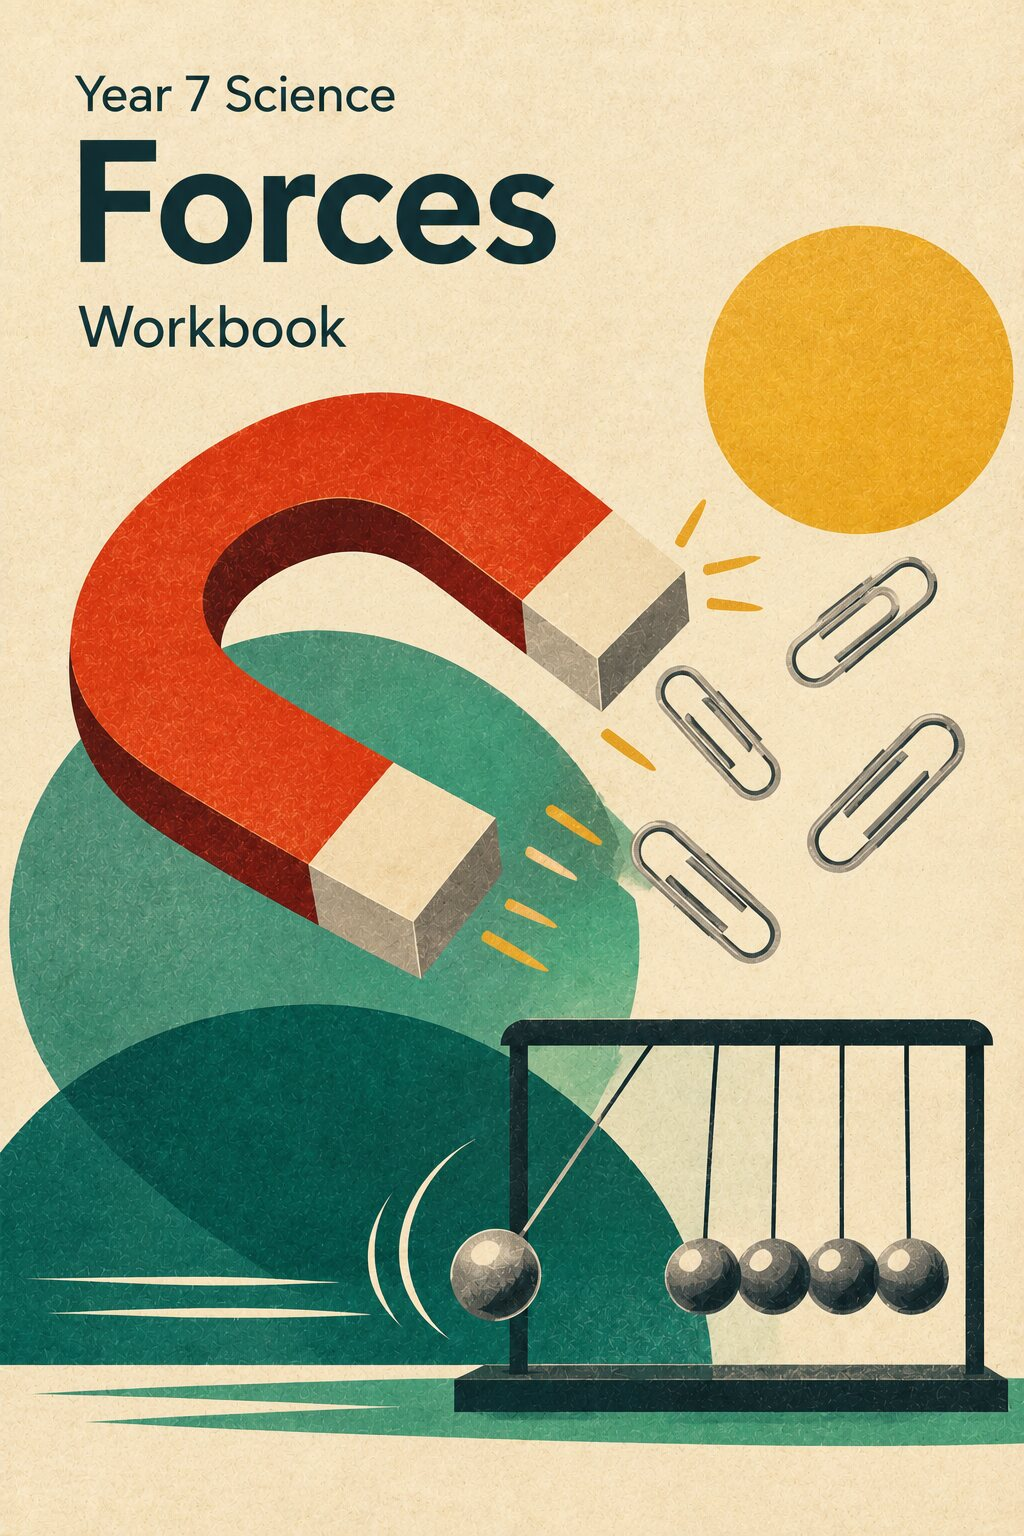
\includegraphics[width=\paperwidth]{../../../covers/forces.jpg}};
  \node[anchor=north east, fill=white, draw=Ink, line width=0.6pt, rounded corners=1.2mm,
        inner xsep=2mm, inner ysep=1.8mm, text width=30mm, font=\headingfont\footnotesize]
    at ([xshift=-4mm, yshift=-4mm]current page.north east)
    {\textbf{Name}\par\vspace{4mm}\hrule\vspace{2mm}\textbf{Class}\par\vspace{4mm}\hrule};
  \node[anchor=south east, fill=white, draw=Ink, line width=0.6pt, rounded corners=1.2mm,
        inner xsep=2.6mm, inner ysep=2mm, font=\headingfont\bfseries, align=right]
    at ([xshift=-4mm, yshift=6mm]current page.south east)
    {Advanced Forces 1\\[-1pt]{\normalfont\headingfont\scriptsize Topics 1--4}};
\end{tikzpicture}
\mbox{}
\clearpage

% ---- Inside cover ---------------------------------------------------------
\thispagestyle{plain}
{\headingfont\bfseries\fontsize{22}{26}\selectfont Advanced Forces}\par\vspace{1mm}
{\headingfont\large Book 1 \textbullet\ Topics 1--4 \textbullet\ Above the Year 7 level}\par\vspace{1mm}
{\small\itshape VC 2.0: VC2S8U13--U15 \textbullet\ VC2S10U15 \textbullet\ VC2S10U17}\par\vspace{4mm}
\textbf{Teacher}\ \hrulefill\par

\begin{countrybox}{Acknowledgement of Country}
This booklet was created on the unceded Country of the Wurundjeri Woi-wurrung people of the Kulin Nation. We acknowledge Elders past, present and emerging.
\end{countrybox}

\begin{infobox}{How this booklet works}
\textbf{Advanced Forces} goes deeper into the ideas of the lesson books: more powerful models, the mathematics behind them, and harder problems that bring several ideas together. Each topic builds on the lessons named under its title. Each opens with its key vocabulary, then:\par\smallskip
\renewcommand{\arraystretch}{1.25}
\begin{tabular}{@{}p{24mm}p{70mm}@{}}
\textbf{Part A} & a reading with comprehension questions \\
\textbf{Part B} & the deeper idea, worked through \\
\textbf{Part C} & practice on your own \\
\textbf{Part D} & a challenge that pulls the ideas together \\
\end{tabular}

\smallskip
\begin{tabular}{@{}p{24mm}p{70mm}@{}}
\textbf{I do} \tagicon{\icodots{1}} & a worked example (solid frame) \\
\textbf{We do} \tagicon{\icodots{2}} & you try one with help (dashed frame) \\
\textbf{Reading} \tagicon{\icoread} & a passage to read (thin frame) \\
\end{tabular}
\end{infobox}

\clearpage
\markboth{Contents}{Contents}
{\headingfont\bfseries\LARGE Contents}\par\vspace{1mm}\noindent\rule{\linewidth}{0.6pt}\par\vspace{2mm}
\renewcommand{\arraystretch}{1.12}
\begin{tabular}{|C{1.1cm}|L{5.2cm}|C{1.7cm}|C{1.4cm}|}
  \hline\thead{Topic} & \thead{Title} & \thead{Deepens lesson} & \thead{Page} \\ \hline
  1 & \hyperlink{lesson.1.1}{Mass, Weight and Gravity Beyond Earth} & 1 & \hyperlink{lesson.1.1}{p.\ \pageref{sec:1}} \\ \hline
  2 & \hyperlink{lesson.2.1}{Net Force, Drag and Terminal Velocity} & 2 & \hyperlink{lesson.2.1}{p.\ \pageref{sec:2}} \\ \hline
  3 & \hyperlink{lesson.3.1}{Force Pairs and Momentum} & 4 & \hyperlink{lesson.3.1}{p.\ \pageref{sec:3}} \\ \hline
  4 & \hyperlink{lesson.4.1}{$F = ma$: Acceleration and Impact} & 5 & \hyperlink{lesson.4.1}{p.\ \pageref{sec:4}} \\ \hline
  5 & \textit{Calculating Energy} & 7 & Book 2 \\ \hline
  6 & \textit{Turning Effects and the Trebuchet} & 9, 10 & Book 2 \\ \hline
  7 & \textit{Optimising Range} & 12 & Book 2 \\ \hline
  --- & \hyperlink{glossary}{Glossary} & & \hyperlink{glossary}{\pageref{sec:glossary}} \\ \hline
\end{tabular}
\renewcommand{\arraystretch}{1}
\clearpage
\setcounter{section}{0}\renewcommand{\lessonart}{1}
\sectiondiv{Mass, Weight and Gravity Beyond Earth}{Gravitational field strength \textbullet{} Why $g$ changes from world to world \textbullet{} Balances and spring scales \textbullet{} Weightless in orbit}\label{sec:1}
\lessoncodes{Deepens Lesson 1 \textbullet{} VC2S8U14 \textbullet{} VC2S10U17}

\vocabhead
\begin{ctab}
\begin{tabular}{|SW{2.91cm}|W{8.05cm}|}
  \hd & \thead{Word} & \thead{Definition (copy from the slide)} \\ \hline
  & \scaf{\textbf{Gravitational field strength}\label{voc:gravitational-field-strength}} & \scaf{The force of gravity on each kilogram of mass at a place, $g$, in newtons per kilogram (N/kg).} \\ \hline
  & \textbf{Gravitational field}\label{voc:gravitational-field} & \cell{a1.v2} \\ \hline
  & \textbf{Free fall}\label{voc:free-fall} & \cell{a1.v3} \\ \hline
  & \textbf{Orbit}\label{voc:orbit} & \cell{a1.v4} \\ \hline
  & \textbf{Apparent weight}\label{voc:apparent-weight} & \cell{a1.v5} \\ \hline
\end{tabular}
\end{ctab}

\lessonpart{A}{Reading and comprehension}{Teal}\label{read:1}

\begin{readingbox}{Reading --- Floating in the Space Station}
Astronauts on the International Space Station float about the cabin, so it is natural to think there is no gravity up there. In fact the station orbits only about 400\,km above the ground, and gravity there is still about 90\% as strong as on Earth's surface. If you could build a tower 400\,km tall and stand on top, you would feel almost your normal weight.

So why do astronauts float? Because the station and everything in it are falling. They are moving sideways so fast --- about 7.7\,km every second --- that as they fall towards Earth, the curved ground falls away beneath them just as quickly. They keep falling around the planet without ever getting closer. This endless fall is an \textbf{orbit}, and things falling freely like this are in \textbf{free fall}.

Every planet and moon is surrounded by a \textbf{gravitational field}, the region where its gravity pulls on masses. The \textbf{gravitational field strength}, $g$, tells you how hard it pulls on each kilogram: 9.8\,N/kg on Earth, 1.6\,N/kg on the Moon. A world with more mass pulls harder, but if it is also much wider, its surface is further from its centre, and the pull there is weaker.

What you \emph{feel} as your weight is really the push of the floor holding you up. In free fall nothing pushes on you, so your \textbf{apparent weight} is zero, even though gravity is still pulling.
\end{readingbox}

\rcreset
\rcqk{a1.c1}{How strong is gravity at the height of the Space Station, compared with on Earth's surface?}{1.6cm}
\rcqk{a1.c2}{Explain why astronauts in the Space Station float, even though gravity is still pulling on them.}{2.4cm}
\rcqk{a1.c3}{Name two things about a planet that decide how strong its gravity is at the surface.}{2cm}
\rcqk{a1.c4}{What is the difference between your weight and your apparent weight?}{2.4cm}

\lessonpart{B}{Theory and examples}{Blue}\label{theory:1}

\subsection{Weight in Different Places}\label{sub:a1.1}

\begin{skillbox}{Weight, mass and $g$}
\[ W = m \times g \qquad m = \frac{W}{g} \qquad g = \frac{W}{m} \]
$W$ is weight (N), $m$ is mass (kg), $g$ is gravitational field strength (N/kg). Your mass is the same everywhere. Your weight changes with $g$.
\end{skillbox}

\begin{ctab}
\begin{tabular}{|C{2.98cm}|C{3.78cm}|C{3.78cm}|}
  \hline\thead{Place} & \thead{$g$ (N/kg)} & \thead{Weight of a 50\,kg student (N)} \\ \hline
  Moon & 1.6 & 80 \\ \hline
  Mars & 3.7 & 185 \\ \hline
  Earth & 9.8 & 490 \\ \hline
  Jupiter (cloud tops) & 24.8 & 1240 \\ \hline
\end{tabular}
\end{ctab}

\begin{workedex}{Finding $g$ on an unknown world}
A probe lands on a moon. A 4\,kg test mass hangs from its spring scale, which reads 5.2\,N. Find $g$ on the moon.

\smallskip
$g = W \div m = 5.2 \div 4 = \mathbf{1.3\ \text{N/kg}}$, a little weaker than on our Moon.
\end{workedex}

\begin{wedo}{Finding $g$ on an unknown world}
The same probe's 4\,kg mass reads 15.2\,N on a second world. Find $g$ there, and say which world in the table it is most like.
\wbox{a1.wd1}{3cm}
\end{wedo}

\subsection{Why $g$ Is Different on Different Worlds}\label{sub:a1.2}

\begin{workedex}{Mass and size together}
Jupiter has about 318 times the mass of Earth, but its $g$ is only about 2.5 times Earth's. Why?

\smallskip
More mass means a stronger pull. But Jupiter is also about 11 times as wide as Earth, so its cloud tops are much further from its centre, and gravity weakens with distance. The two effects work against each other, so the extra mass is mostly cancelled out by the extra distance.
\end{workedex}

\begin{wedo}{Mass and size together}
Mars has about one-tenth of Earth's mass and about half of Earth's width. Use both facts to explain why $g$ on Mars (3.7\,N/kg) is less than Earth's, but not as small as one-tenth of it.
\abox{a1.wd2}{4.5cm}
\end{wedo}

\lessonpart{C}{Practice}{Amber}\label{prac:1}

\needspace{10\baselineskip}
\task An astronaut has a mass of 75\,kg.
\pt{a}Find her weight on Earth.
\wbox{1.x13a}{2.0cm}
\pt{b}Find her weight on the Moon.
\wbox{1.x13b}{2.0cm}
\pt{c}Explain why she can jump much higher on the Moon, even though her mass has not changed.
\abox{1.x13c}{2.0cm}


\needspace{10\baselineskip}
\task A suitcase has a weight of 196\,N on Earth.
\pt{a}Find its mass.
\wbox{1.x14a}{2.0cm}
\pt{b}Find its weight on the Moon.
\wbox{1.x14b}{2.0cm}

\needspace{10\baselineskip}
\task A bathroom scale really measures \emph{force}, but it is labelled in kilograms. A 60\,kg student reads 60\,kg on it on Earth. Predict what the same scale would read on the Moon, and explain why the scale is not really measuring mass.
\abox{1.x15}{3.0cm}

\needspace{10\baselineskip}
\task On Mars, $g = 3.7$\,N/kg. A 10\,kg backpack is carried on Earth ($g = 9.8$\,N/kg), on the Moon ($g = 1.6$\,N/kg) and on Mars.
\pt{a}Calculate the backpack's weight in each place.
\wbox{1.x16a}{2.0cm}
\pt{b}Rank the three places from easiest to hardest to carry the backpack, and explain your ranking.
\abox{1.x16b}{2.0cm}

\needspace{10\baselineskip}
\task A rock hangs from a spring scale on Earth, and the scale reads 4.9\,N. Use $g = 9.8$\,N/kg on Earth and $g = 1.6$\,N/kg on the Moon.
\pt{a}Find the mass of the rock.
\wbox{1.x17a}{2.0cm}
\pt{b}Find what the same spring scale would read if the rock were hung from it on the Moon.
\wbox{1.x17b}{2.0cm}

\needspace{10\baselineskip}
\task A \emph{balance} compares an object with known masses. A \emph{spring scale} measures the pull of gravity on the object. Explain why a balance gives the same result on the Moon as on Earth, but a spring scale does not.
\abox{1.x18}{3.2cm}

\needspace{10\baselineskip}
\task Magnets can push or pull without touching. Describe a quick test you could do with a magnet, a paperclip and a sheet of paper to show that magnetic force acts \emph{through} the paper. Say what you would do and what you would expect to see.
\abox{1.x19}{3.4cm}


\needspace{10\baselineskip}
\task A student stands on bathroom scales in a lift. Explain what happens to the reading as the lift starts to speed up going \emph{up}, and why. (Hint: what must the floor do to make the student speed up?)
\abox{a1.t1}{5cm}

\lessonpart{D}{Challenge}{Violet}\label{ext:1}

\task The Space Station travels at 7.7\,km/s. Explain, step by step, why the astronauts inside it are falling all the time but never land. Then explain what would happen to the station if it suddenly stopped moving sideways.
\abox{a1.ch}{7cm}

\clearpage
% ══════════════════════════════════════════════════════════════════════════════
%  TOPIC 2 — NET FORCE, DRAG AND TERMINAL VELOCITY          (deepens Lesson 2)
% ══════════════════════════════════════════════════════════════════════════════
\setcounter{section}{1}\renewcommand{\lessonart}{2}
\sectiondiv{Net Force, Drag and Terminal Velocity}{Drag grows with speed \textbullet{} Four forces on a vehicle \textbullet{} The skydiver's fall, stage by stage}\label{sec:2}
\lessoncodes{Deepens Lesson 2 \textbullet{} VC2S8U14 \textbullet{} VC2S10U17}

\vocabhead
\begin{ctab}
\begin{tabular}{|SW{2.91cm}|W{8.05cm}|}
  \hd & \thead{Word} & \thead{Definition (copy from the slide)} \\ \hline
  & \scaf{\textbf{Drag}\label{voc:drag}} & \scaf{A force that pushes against an object moving through air or water; air resistance is drag in air.} \\ \hline
  & \textbf{Terminal velocity}\label{voc:terminal-velocity} & \cell{a2.v2} \\ \hline
  & \textbf{Streamlined}\label{voc:streamlined} & \cell{a2.v3} \\ \hline
  & \textbf{Driving force}\label{voc:driving-force} & \cell{a2.v4} \\ \hline
  & \textbf{Resistive force}\label{voc:resistive-force} & \cell{a2.v5} \\ \hline
\end{tabular}
\end{ctab}

\lessonpart{A}{Reading and comprehension}{Teal}\label{read:2}

\begin{readingbox}{Reading --- The Fastest Fall}
In 2012 Felix Baumgartner jumped from a balloon 39\,km above New Mexico. In the thin air up there, almost nothing held him back, and he fell faster than the speed of sound --- over 1300\,km/h. A skydiver jumping from a plane at 4\,km never gets close to that. Why?

The answer is \textbf{drag}. Drag is the force of the air pushing against a moving object, and it grows as the object goes faster. At first a falling skydiver is slow, drag is small, and the net force is almost their whole weight, so they speed up quickly. As they speed up, drag grows, the net force shrinks, and they speed up less and less. Eventually drag is as big as their weight. The forces are balanced, and they fall at a steady top speed: their \textbf{terminal velocity}, about 200\,km/h for a skydiver lying flat.

Thick air means lots of drag. Baumgartner's air was so thin that drag stayed small, so his terminal velocity was huge. Shape matters too: a \textbf{streamlined} shape, like a diving falcon's, slips through the air with less drag.

Cars face the same battle. The engine provides a \textbf{driving force}; drag and friction are \textbf{resistive forces}. A car's top speed is reached when the resistive forces grow to match the driving force.
\end{readingbox}

\rcreset
\rcqk{a2.c1}{What happens to drag as an object moves faster?}{1.6cm}
\rcqk{a2.c2}{Why does a skydiver speed up quickly at first, then less and less?}{2.4cm}
\rcqk{a2.c3}{What is terminal velocity, and when is it reached?}{2.2cm}
\rcqk{a2.c4}{Why could Baumgartner fall so much faster than an ordinary skydiver?}{2.2cm}

\lessonpart{B}{Theory and examples}{Blue}\label{theory:2}

\subsection{The Skydiver, Stage by Stage}\label{sub:a2.1}

\begin{center}
\begin{fitbox}\begin{tikzpicture}[font=\small]
  \draw[-{Stealth[length=5pt]}, line width=0.8pt] (0,0) -- (9.2,0) node[below left, font=\scriptsize]{time};
  \draw[-{Stealth[length=5pt]}, line width=0.8pt] (0,0) -- (0,4.4) node[above right, font=\scriptsize]{speed};
  \draw[line width=1.4pt] (0,0) .. controls (1.2,2.6) and (2.2,3.4) .. (3.6,3.5) -- (5,3.5);
  \draw[line width=1.4pt] (5,3.5) .. controls (5.3,1.6) and (5.6,1.3) .. (6.4,1.2) -- (8.8,1.2);
  \draw[densely dotted] (0,3.5) node[left, font=\scriptsize]{terminal} -- (3.6,3.5);
  \draw[densely dotted] (0,1.2) node[left, font=\scriptsize]{new terminal} -- (6.4,1.2);
  \foreach \x/\y/\l in {0.7/1.55/A, 4.3/3.85/B, 5.6/2.4/C, 7.6/1.55/D}{\node[draw, circle, inner sep=1pt, font=\scriptsize\bfseries, fill=white] at (\x,\y) {\l};}
  \node[font=\scriptsize, anchor=west] at (5.1,3.75) {parachute opens};
  \draw[-{Stealth[length=4pt]}] (5.6,3.6) -- (5.05,3.5);
\end{tikzpicture}\end{fitbox}
\figcap{Speed of a skydiver: A speeding up, B terminal velocity, C parachute opens, D a new, slower terminal velocity.}
\end{center}

\begin{workedex}{Explaining stage A and stage B}
\textbf{Stage A:} weight (down) is bigger than drag (up). The net force is downwards, so the skydiver speeds up. As speed grows, drag grows, so the net force gets smaller.\\
\textbf{Stage B:} drag has grown until it equals weight. The forces are balanced, the net force is zero, so the speed stays the same: terminal velocity.
\end{workedex}

\begin{wedo}{Explaining stage C and stage D}
Use the words \emph{drag}, \emph{weight} and \emph{net force} to explain what happens to the skydiver's speed at stage C, when the parachute opens, and why it levels off again at stage D.
\abox{a2.wd1}{5cm}
\end{wedo}

\subsection{Four Forces on a Vehicle}\label{sub:a2.2}

\begin{workedex}{A car's top speed}
A car's engine gives a driving force of 3000\,N. At 80\,km/h the resistive forces total 1800\,N.

\smallskip
Net force $= 3000 - 1800 = \mathbf{1200\ \text{N}}$ forwards, so the car is still speeding up. As it goes faster the resistive forces grow. It reaches top speed when they reach 3000\,N, and the net force is zero.
\end{workedex}

\begin{wedo}{A car's top speed}
A cyclist pedals with a driving force of 150\,N. At 30\,km/h the resistive forces are 150\,N. What is the net force, and what is happening to the cyclist's speed? Suggest one way the cyclist could reach a higher top speed without pedalling harder.
\abox{a2.wd2}{4.5cm}
\end{wedo}

\lessonpart{C}{Practice}{Amber}\label{prac:2}

\needspace{10\baselineskip}
\task Sam says: \emph{``A hockey puck sliding across ice at a steady speed must have an unbalanced force pushing it forwards.''} Is Sam right? Use a free body diagram and the idea of net force to explain.
\abox{2.x17}{3.4cm}

\needspace{14\baselineskip}
\task A skydiver jumps from a plane. Draw a free body diagram for each moment below. Then explain why air resistance grows, and why the skydiver eventually stops speeding up.
\pt{i}just after jumping
\pt{ii}while still speeding up
\pt{iii}at terminal velocity

\vspace{3pt}
\par\noindent\drawk{2.x18i}{4.2cm}{\textbf{(i)} just after jumping}
\par\noindent\drawk{2.x18ii}{4.2cm}{\textbf{(ii)} speeding up}
\par\noindent\drawk{2.x18iii}{4.2cm}{\textbf{(iii)} terminal velocity}\par
\abox{2.x18-why}{2.6cm}

\needspace{10\baselineskip}
\task A car has a driving force of 4500\,N and a total resistive force of 1200\,N.
\pt{a}Calculate the net force.
\wbox{2.x19a}{2.0cm}
\pt{b}State which way the car accelerates.
\abox{2.x19b}{2.0cm}
\pt{c}Suggest one way the driver could make the forces balanced.
\abox{2.x19c}{2.0cm}

\needspace{10\baselineskip}
\task A 1200\,kg car has a driving force of 4800\,N. Air resistance and friction total 1500\,N.
\pt{a}Find the net force.
\wbox{2.x20a}{2.0cm}
\pt{b}Use $F = ma$ (acceleration = net force $\div$ mass) to find the acceleration.
\wbox{2.x20b}{2.0cm}
\pt{c}The driving force rises to 6000\,N --- find the new acceleration.
\wbox{2.x20c}{2.0cm}
\needspace{16\baselineskip}
\task A car drives along a flat road at a steady 60\,km/h. Draw a free body diagram for the car showing four forces: weight, the normal force, the driving force and the total resistive force. Show which pairs of forces are balanced.

\vspace{3pt}
\drawk{2.x21}{4.6cm}{
\textit{\color{MidGrey}Draw your force diagram here.}
}

\needspace{10\baselineskip}
\task A 2\,kg ball is falling. Air resistance pushes up on it with 5\,N. Use $W = mg$ with $g = 9.8$\,N/kg.
\pt{a}Find the weight of the ball.
\wbox{2.x22a}{2.0cm}
\pt{b}Find the size and direction of the net force.
\wbox{2.x22b}{2.0cm}
\pt{c}Is the ball speeding up, slowing down or moving at a steady speed? Explain.
\abox{2.x22c}{2.0cm}

\needspace{10\baselineskip}
\task A loaded truck and a small car are both travelling at the same speed. Explain, using the idea of net force, why the truck needs a much bigger braking force to stop in the same distance.
\abox{2.x23}{3.0cm}


\lessonpart{D}{Challenge}{Violet}\label{ext:2}

\task A falcon dives for prey with its wings folded back. A second falcon of the same mass dives with its wings spread out. Predict which reaches the greater terminal velocity, and explain why, using the forces acting on each bird. Sketch both lines on one speed--time graph.
\abox{a2.ch}{5cm}
\drawk{a2.ch-graph}{5cm}{}

\clearpage
% ══════════════════════════════════════════════════════════════════════════════
%  TOPIC 3 — FORCE PAIRS AND MOMENTUM                       (deepens Lesson 4)
% ══════════════════════════════════════════════════════════════════════════════
\setcounter{section}{2}\renewcommand{\lessonart}{4}
\sectiondiv{Force Pairs and Momentum}{Third Law pair or balanced pair? \textbullet{} Momentum \textbullet{} Pushing apart: recoil}\label{sec:3}
\lessoncodes{Deepens Lesson 4 \textbullet{} VC2S8U14 \textbullet{} VC2S10U17}

\vocabhead
\begin{ctab}
\begin{tabular}{|SW{2.91cm}|W{8.05cm}|}
  \hd & \thead{Word} & \thead{Definition (copy from the slide)} \\ \hline
  & \scaf{\textbf{Momentum}\label{voc:momentum}} & \scaf{How hard it is to stop a moving object: mass $\times$ velocity, in kg\,m/s.} \\ \hline
  & \textbf{Third Law pair}\label{voc:third-law-pair} & \cell{a3.v2} \\ \hline
  & \textbf{Recoil}\label{voc:recoil} & \cell{a3.v3} \\ \hline
  & \textbf{Conservation of momentum}\label{voc:conservation-of-momentum} & \cell{a3.v4} \\ \hline
\end{tabular}
\end{ctab}

\lessonpart{A}{Reading and comprehension}{Teal}\label{read:3}

\begin{readingbox}{Reading --- The Kick of a Fire Hose}
A fire hose at full pressure can knock a firefighter over, so it takes two or three people to hold one. The hose pushes water forwards out of the nozzle, and by Newton's Third Law the water pushes the hose backwards with an equal force. This backwards push is called \textbf{recoil}. A cannon recoils when it fires, and a skateboard rolls backwards when you jump off its front.

Newton's Third Law pairs always act on two \emph{different} objects --- here, the hose and the water. That is why they do not cancel out. Forces only cancel when they act on the \emph{same} object.

Scientists use \textbf{momentum} to describe recoil. Momentum is mass times velocity: a heavy, fast object has a lot of momentum. When two things push apart from rest, they end up with equal momentum in opposite directions, so the total is still zero. This is the law of \textbf{conservation of momentum}. A small, light object shoots away fast; a big, heavy one moves off slowly.
\end{readingbox}

\rcreset
\rcqk{a3.c1}{Why does a fire hose push backwards on the firefighters?}{2.2cm}
\rcqk{a3.c2}{Why do the two forces in a Third Law pair not cancel each other out?}{2.2cm}
\rcqk{a3.c3}{What two things decide how much momentum an object has?}{1.6cm}
\rcqk{a3.c4}{Two objects push apart from rest. Which one moves faster, the light one or the heavy one?}{1.8cm}

\lessonpart{B}{Theory and examples}{Blue}\label{theory:3}

\subsection{Third Law Pair or Balanced Pair?}\label{sub:a3.1}

\begin{skillbox}{The three tests for a Third Law pair}
\textbf{1.} The two forces act on \emph{two different objects}. \quad \textbf{2.} They are the \emph{same type} of force (both gravity, both contact \dots). \quad \textbf{3.} They are equal in size and opposite in direction.

A \textbf{balanced pair} passes only test 3: both forces act on the same object.
\end{skillbox}

\begin{workedex}{A book on a table}
\textbf{Earth pulls the book down (weight)} and \textbf{the table pushes the book up (normal force)}: both act on the book, and they are different types. This is a \emph{balanced pair}, not a Third Law pair.

\smallskip
The Third Law partner of the book's weight is \textbf{the book pulling the Earth up} --- same type (gravity), on a different object (the Earth).
\end{workedex}

\begin{wedo}{A swimmer}
A swimmer pushes backwards on the water with her hands. Name the Third Law partner of this force, and use the three tests to show it is a Third Law pair.
\abox{a3.wd1}{4.5cm}
\end{wedo}

\subsection{Momentum and Recoil}\label{sub:a3.2}

\begin{skillbox}{Momentum}
\[ p = m \times v \]
$p$ is momentum (kg\,m/s), $m$ is mass (kg), $v$ is velocity (m/s). When two objects push apart from rest: \quad $m_1 v_1 = m_2 v_2$ (in opposite directions).
\end{skillbox}

\begin{workedex}{Two skaters}
A 60\,kg skater and a 40\,kg skater stand still on ice and push apart. The 60\,kg skater moves off at 2\,m/s. How fast does the 40\,kg skater move?

\smallskip
Momentum of the first skater $= 60 \times 2 = 120$\,kg\,m/s.\\
The second must have 120\,kg\,m/s the other way: $v = 120 \div 40 = \mathbf{3\ \text{m/s}}$.
\end{workedex}

\begin{wedo}{A cannon}
A 500\,kg cannon fires a 10\,kg ball at 100\,m/s. Find the ball's momentum, then the speed at which the cannon recoils.
\wbox{a3.wd2}{3.5cm}
\end{wedo}

\lessonpart{C}{Practice}{Amber}\label{prac:3}

\needspace{10\baselineskip}
\task Jess says: \emph{``The weight of a book on a table and the normal force from the table are a Third Law pair, because they are equal and opposite.''} Is Jess right? Explain, and name the true reaction force to each of the two forces.
\abox{4.x15}{2.8cm}

\needspace{12\baselineskip}
\task For each pair of forces, decide whether it is a Third Law pair. Write \textbf{YES} or \textbf{NO}, and explain how you decided.
\pt{i}The Earth pulls a book down; the book pulls the Earth up.
\abox{4.x16i}{2.0cm}
\pt{ii}A rope pulls a sledge forwards; friction from the snow pulls the sledge backwards.
\abox{4.x16ii}{2.0cm}
\pt{iii}A swimmer pushes the water backwards; the water pushes the swimmer forwards.
\abox{4.x16iii}{2.0cm}

\needspace{10\baselineskip}
\task A horse pulls a cart. By the Third Law, the cart pulls back on the horse with an equal force. Liam says: \emph{``So the forces cancel out, and the horse can never get the cart moving.''} Explain Liam's mistake. \textit{(Hint: draw a free body diagram for the horse alone. What pushes the horse forwards?)}
\abox{4.x17}{3.0cm}

\needspace{10\baselineskip}
\task An astronaut on a spacewalk is floating 10\,m from the Space Station, not moving. Her safety line has come loose, but she is holding a heavy toolbox.
\pt{a}Explain how she can use the Third Law to start moving back towards the station.
\abox{4.x18a}{2.0cm}
\pt{b}Once she is moving, does she need to keep doing anything to keep moving? Use the First Law.
\abox{4.x18b}{2.0cm}

\needspace{10\baselineskip}
\task An apple falls from a tree. The Earth pulls the apple down with a force of 1\,N.
\pt{a}What is the reaction force? Give its size and direction, and say what it acts on.
\abox{4.x19a}{2.0cm}
\pt{b}The two forces are the same size. So why do we see the apple move towards the Earth, and not the Earth move towards the apple? Use the idea of inertia.
\abox{4.x19b}{2.0cm}

\needspace{10\baselineskip}
\task Two skaters stand still on ice and push each other apart. Skater A has twice the mass of skater B.
\pt{a}Compare the sizes of the forces on the two skaters.
\abox{4.x20a}{2.0cm}
\pt{b}Which skater moves away faster? Explain, using the idea of inertia.
\abox{4.x20b}{2.0cm}

\needspace{10\baselineskip}
\task A waiter carries a full cup of water on a tray.
\pt{a}The waiter suddenly moves the tray forwards. Which way does the water spill? Explain.
\abox{4.x21a}{2.0cm}
\pt{b}Later, walking at a steady speed, the waiter suddenly stops. Which way does the water spill now? Explain.
\abox{4.x21b}{2.0cm}
\pt{c}Use the First Law to explain why moving the tray smoothly stops the water spilling.
\abox{4.x21c}{2.0cm}


\lessonpart{D}{Challenge}{Violet}\label{ext:3}

\task A rocket in deep space has nothing to push against, yet it can still speed up. Use Newton's Third Law \emph{and} the idea of momentum to explain how. Then explain why a rocket that throws its exhaust out faster gains more speed from the same amount of fuel.
\abox{a3.ch}{7cm}

\clearpage
% ══════════════════════════════════════════════════════════════════════════════
%  TOPIC 4 — F = ma: ACCELERATION AND IMPACT                (deepens Lesson 5)
% ══════════════════════════════════════════════════════════════════════════════
\setcounter{section}{3}\renewcommand{\lessonart}{5}
\sectiondiv{\texorpdfstring{$F = ma$}{F = ma}: Acceleration and Impact}{Net force first \textbullet{} Acceleration from speeds and time \textbullet{} Lifts \textbullet{} Impacts and crumple zones}\label{sec:4}
\lessoncodes{Deepens Lesson 5 \textbullet{} VC2S8U14 \textbullet{} VC2S10U17}

\vocabhead
\begin{ctab}
\begin{tabular}{|SW{2.91cm}|W{8.05cm}|}
  \hd & \thead{Word} & \thead{Definition (copy from the slide)} \\ \hline
  & \scaf{\textbf{Change in velocity}\label{voc:change-in-velocity}} & \scaf{Final velocity minus starting velocity, $\Delta v$, in m/s.} \\ \hline
  & \textbf{Deceleration}\label{voc:deceleration} & \cell{a4.v2} \\ \hline
  & \textbf{Impact force}\label{voc:impact-force} & \cell{a4.v3} \\ \hline
  & \textbf{Crumple zone}\label{voc:crumple-zone} & \cell{a4.v4} \\ \hline
\end{tabular}
\end{ctab}

\lessonpart{A}{Reading and comprehension}{Teal}\label{read:4}

\begin{readingbox}{Reading --- Cars Built to Crush}
A modern car is designed to be destroyed in a crash. Its front and back are \textbf{crumple zones}: parts built to fold up slowly, like a drink can being squashed. This might sound like bad engineering, but it saves lives.

In a crash, the car and the people in it must lose all their speed. Newton's Second Law says that the force needed to change an object's motion depends on how quickly the change happens. If a car stops dead against a wall in a few thousandths of a second, the people inside feel an enormous \textbf{impact force}. If the front crumples and the stop takes ten times as long, the force on them is ten times smaller.

Slowing down is called \textbf{deceleration}. Seatbelts stretch a little, airbags squash, and crumple zones fold, all for the same reason: to make the deceleration take longer, so the force is smaller. Bicycle helmets, the sand pit in long jump and the bend in your knees when you land from a jump all work the same way.
\end{readingbox}

\rcreset
\rcqk{a4.c1}{What is a crumple zone, and why is it built to crush?}{2.2cm}
\rcqk{a4.c2}{How does making a stop take longer change the force on the people in the car?}{2.2cm}
\rcqk{a4.c3}{Give two other examples that work in the same way as a crumple zone.}{2cm}

\lessonpart{B}{Theory and examples}{Blue}\label{theory:4}

\subsection{Acceleration From Speeds and Time}\label{sub:a4.1}

\begin{skillbox}{Two steps}
\textbf{Step 1:} \quad $a = \dfrac{\Delta v}{t} = \dfrac{\text{final velocity} - \text{starting velocity}}{\text{time}}$ \qquad \textbf{Step 2:} \quad $F = m \times a$ \quad (this $F$ is the \emph{net} force).

A negative acceleration is a deceleration.
\end{skillbox}

\begin{workedex}{A car braking}
A 1000\,kg car slows from 20\,m/s to 0\,m/s in 4\,s.

\smallskip
$a = (0 - 20) \div 4 = -5$\,m/s$^2$ \quad (a deceleration of 5\,m/s$^2$)\\
$F = 1000 \times 5 = \mathbf{5000\ \text{N}}$ backwards, from the brakes and road.
\end{workedex}

\begin{wedo}{A sprinter}
A 60\,kg sprinter speeds up from 0 to 9\,m/s in 1.5\,s. Find her acceleration, then the net force on her.
\wbox{a4.wd1}{3.5cm}
\end{wedo}

\subsection{Impacts: the Same Change, a Longer Time}\label{sub:a4.2}

\begin{workedex}{Crash test}
A 70\,kg crash-test dummy stops from 15\,m/s. Compare a stop in 0.01\,s (rigid car) with a stop in 0.1\,s (crumple zone and airbag).

\smallskip
\textbf{Rigid:} $a = 15 \div 0.01 = 1500$\,m/s$^2$; $F = 70 \times 1500 = \mathbf{105\,000\ \text{N}}$\\
\textbf{Crumple:} $a = 15 \div 0.1 = 150$\,m/s$^2$; $F = 70 \times 150 = \mathbf{10\,500\ \text{N}}$, ten times smaller.
\end{workedex}

\begin{wedo}{Landing from a jump}
A 50\,kg student jumps off a wall and hits the ground at 4\,m/s. Find the force on her legs if she lands stiff-legged and stops in 0.02\,s, and if she bends her knees and stops in 0.2\,s.
\wbox{a4.wd2}{4.5cm}
\end{wedo}

\lessonpart{C}{Practice}{Amber}\label{prac:4}

\needspace{10\baselineskip}
\task Ahmed pushes a 20\,kg crate with a force of 60\,N, but it does not move. He says: \emph{``$F = ma$ means it should accelerate at 3\,m/s$^2$, so the formula must be wrong.''} Explain Ahmed's mistake, and find the size of the friction force on the crate.
\wbox{5.x15}{3.0cm}

\needspace{10\baselineskip}
\task Mia pushes a 50\,kg crate across the floor. Friction on the crate is 40\,N. She says: \emph{``If I push twice as hard, the crate will speed up twice as fast.''}
\pt{a}Find the acceleration when she pushes with 100\,N.
\wbox{5.x16a}{2.0cm}
\pt{b}Find the acceleration when she pushes with 200\,N.
\wbox{5.x16b}{2.0cm}
\pt{c}Is Mia right? Explain, using the idea of net force.
\abox{5.x16c}{2.0cm}

\needspace{10\baselineskip}
\task A rocket's engines push exhaust gas downwards with a force of 500\,000\,N, and the gas pushes the rocket upwards with the same force. The rocket has a mass of 20\,000\,kg. Use $g = 9.8$\,N/kg.
\pt{a}Find the rocket's weight.
\wbox{5.x17a}{2.0cm}
\pt{b}Find the net force on the rocket at lift-off.
\wbox{5.x17b}{2.0cm}
\pt{c}Find its acceleration.
\wbox{5.x17c}{2.0cm}
\pt{d}Which of Newton's laws explains (i) the upward push of the gas, and (ii) the size of the acceleration?
\abox{5.x17d}{2.0cm}

\needspace{10\baselineskip}
\task A lift and its passengers have a total mass of 800\,kg. The cable pulls the lift upwards with a force of 8640\,N. Use $g = 9.8$\,N/kg.
\pt{a}Find the weight of the lift and its passengers.
\wbox{5.x18a}{2.0cm}
\pt{b}Find the size and direction of the net force.
\wbox{5.x18b}{2.0cm}
\pt{c}Find the acceleration of the lift.
\wbox{5.x18c}{2.0cm}

\needspace{10\baselineskip}
\task A cyclist speeds up from 2\,m/s to 8\,m/s in 4\,s. The cyclist and bicycle have a total mass of 80\,kg.
\pt{a}Calculate the acceleration, using $a = \Delta v \div t$ (change in speed $\div$ time).
\wbox{5.x19a}{2.0cm}
\pt{b}Calculate the net force on the cyclist and bicycle.
\wbox{5.x19b}{2.0cm}
\pt{c}Air resistance and friction total 40\,N. Find the force the cyclist must supply by pedalling.
\wbox{5.x19c}{2.0cm}

\needspace{10\baselineskip}
\task A 0.045\,kg golf ball is struck and leaves the tee at 60\,m/s. The club is in contact with the ball for 0.0005\,s.
\pt{a}Calculate the acceleration of the ball, using $a = \Delta v \div t$ (change in speed $\div$ time).
\wbox{5.x20a}{2.0cm}
\pt{b}Calculate the force applied by the club.
\wbox{5.x20b}{2.0cm}
\pt{c}Calculate the ball's weight, and comment on how the force from the club compares with it.
\wbox{5.x20c}{2.0cm}

\needspace{10\baselineskip}
\task In the trebuchet investigation at the end of this unit, a sling swings a 0.05\,kg projectile. While it is being swung, the net force on the projectile is 2\,N.
\pt{a}Find the projectile's acceleration.
\wbox{5.x21a}{2.0cm}
\pt{b}The sling pulls on the projectile. Describe the reaction force.
\abox{5.x21b}{2.0cm}
\pt{c}Once the projectile leaves the sling, nothing pushes it forwards. Explain why it keeps moving forwards, and name the force that brings it back to the ground.
\abox{5.x21c}{2.0cm}


\lessonpart{D}{Challenge}{Violet}\label{ext:4}

\task You are designing packaging to post a 0.4\,kg glass vase. In a drop, it hits the ground at 5\,m/s, and it breaks if the force on it is more than 200\,N.
\pt{a}What is the shortest stopping time that keeps the force below 200\,N?
\wbox{a4.ch-a}{3cm}
\pt{b}Describe packaging that would make the stop take at least that long, and explain how it works.
\abox{a4.ch-b}{4.5cm}

\clearpage
% ══════════════════════════════════════════════════════════════════════════════
%  TOPIC 5 — CALCULATING ENERGY                             (deepens Lesson 7)
% ══════════════════════════════════════════════════════════════════════════════

\clearpage\markboth{Glossary}{Glossary}\hypertarget{glossary}{}\pdfbookmark[1]{Glossary}{glossarybm}
{\headingfont\bfseries\LARGE Glossary}\label{sec:glossary}\par\vspace{1mm}\noindent\rule{\linewidth}{0.6pt}\par
{\small Every key word in this booklet and the page it is introduced on.}\par\smallskip
\renewcommand{\arraystretch}{1.3}
\begin{longtable}{|>{\RaggedRight}p{34mm}|p{9mm}|p{\dimexpr\linewidth-43mm-6\tabcolsep-4\arrayrulewidth-1pt\relax}|}
\hline \rule{0pt}{4mm}\headingfont\bfseries Word & \headingfont\bfseries Page & \headingfont\bfseries In my own words \\ \hline \endhead
  Apparent weight & \pageref{voc:apparent-weight} & \\ \hline
  Change in velocity & \pageref{voc:change-in-velocity} & \\ \hline
  Conservation of momentum & \pageref{voc:conservation-of-momentum} & \\ \hline
  Crumple zone & \pageref{voc:crumple-zone} & \\ \hline
  Deceleration & \pageref{voc:deceleration} & \\ \hline
  Drag & \pageref{voc:drag} & \\ \hline
  Driving force & \pageref{voc:driving-force} & \\ \hline
  Free fall & \pageref{voc:free-fall} & \\ \hline
  Gravitational field & \pageref{voc:gravitational-field} & \\ \hline
  Gravitational field strength & \pageref{voc:gravitational-field-strength} & \\ \hline
  Impact force & \pageref{voc:impact-force} & \\ \hline
  Momentum & \pageref{voc:momentum} & \\ \hline
  Orbit & \pageref{voc:orbit} & \\ \hline
  Recoil & \pageref{voc:recoil} & \\ \hline
  Resistive force & \pageref{voc:resistive-force} & \\ \hline
  Streamlined & \pageref{voc:streamlined} & \\ \hline
  Terminal velocity & \pageref{voc:terminal-velocity} & \\ \hline
  Third Law pair & \pageref{voc:third-law-pair} & \\ \hline
\end{longtable}
\padtofour
\end{document}
